\chapter{Geometrical Acoustics Rendering Pipelines for Augmented Acoustics}\label{ch:acousticrendering} % If you're changing this, update Section 1.6

This chapter shows the prototyping of a bespoke acoustic rendering pipeline for dynamic virtual environments that integrates material recognition that can extend to immersive technology applications. The design process started with a simplistic form of acoustic rendering, using a standard method to approximate reverb, and expanded towards a bespoke ray tracing-based system that handles dynamic geometry.

\section{Image Source-Based Rendering}
The initial design of the rendering framework employs the classic Image-Source Model (ISM) \citep{savioja1999creating, allen1979image} to compute reflection paths in a given virtual scene reconstruction, as illustrated in Figure~\ref{fig:image-source-pipeline}. The \emph{geometry reduction} component of this pipeline decomposes the virtual scene into a simpler cuboid volume. Vision-based material recognition techniques are used to understand the acoustic characteristics of surfaces in the input scene; these characteristics are then mapped onto the appropriate surfaces of the acoustic volume representing the given virtual scene. Finally, the ISM is supplied with spatial information on emitters and listeners to produce RIRs from the acoustic volume.\par

\begin{figure}[htb]
    \centering
    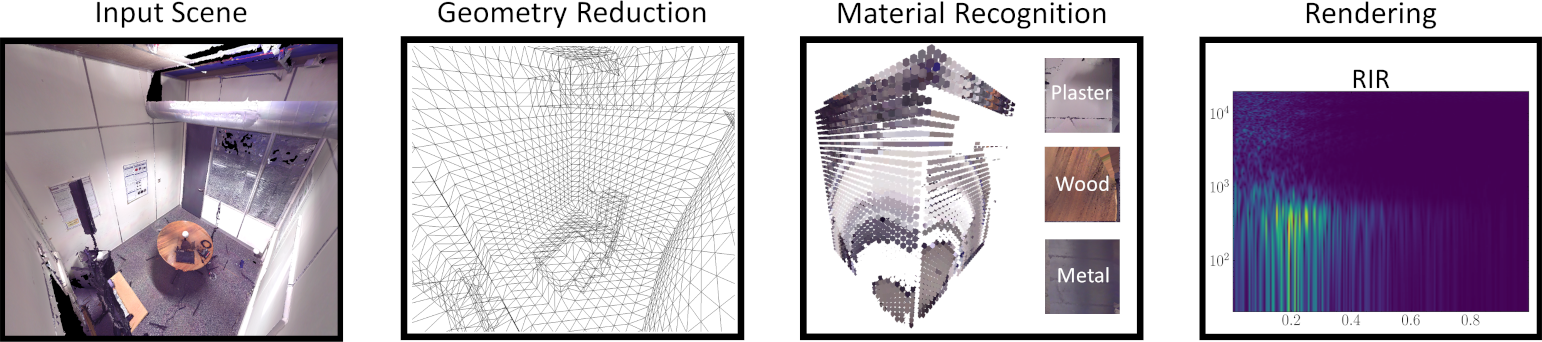
\includegraphics[width=1\linewidth]{image-source-renderer}
    \caption{The Image Source Model (ISM) pipeline showing the four stages of the rendering process (left to right): an input scene is used as input; a geometry reduction process simplifies the complexity of the virtual environment to a cuboid volume; based on portions of the geometry dictated by the cuboid volume, materials of the input environment are determined; materials and simplified geometry provide input to the ISM to produce reverberation responses.}
\label{fig:image-source-pipeline}
\end{figure}

\subsection{Geometry Reduction}
The \emph{geometry reduction}, Figure~\ref{fig:image-source-pipeline}, generates a binary field, sampling from the input geometry at a given number of points. The field shapes the acoustic volume using a marching cubes algorithm, where each cell captures the appearance of surfaces from textures associated with meshes of the input geometry. A cuboid volume encapsulating the reconstructed surface determines the dimensions of the acoustic space simulated with the ISM. Using the vision-based techniques discussed in Chapter~\ref{ch:Materials} to analyse surface appearance, acoustic materials are inferred per image patch, effectively mapping acoustic materials to the surface of the acoustic volume.\par
Input geometry is decomposed into a binary field expressed as $\mathbf{B} = (b_{x,y,z}) \in \{ 0, 1 \}^{P}$, where $P$ is the number of points sampled across the three dimensions. The definition of $\mathbf{B}$ is relevant to the quality of the resulting acoustic simulation and determines the accuracy of the acoustic material recognition, discussed in the following section. Given the set of input meshes from the complex scenes, we define an Axis-Aligned Bounding Box (AABB) encapsulating all vertices of a given scene object, normalising their coordinates to the $[-1, +1]$ range. Values in $\mathbf{B}$ equate to $1$ whenever a cell is within the coordinates of any AABB defined and to $0$ otherwise. The term AABBs will refer to the collection of all bounding boxes associated with scene objects throughout the rest of this Section. A multi-threaded implementation of the marching cubes algorithm \citep{bourke1994polygonising, lengyel2019foundations} shapes the binary field into a volume, representing the acoustic environment for reflection path computation. In this process, the use of the AABB to probe the input scene objects introduces error in cases with concave geometry, which negatively correlates to the resolution of $\mathbf{B}$ as collision checks with AABBs increase with the number of cells. A cuboid encapsulating the reconstructed surface from the marching cubes determines the ISM volume for the reflection computation stage.\par

\begin{figure}[htb]
    \centering 
    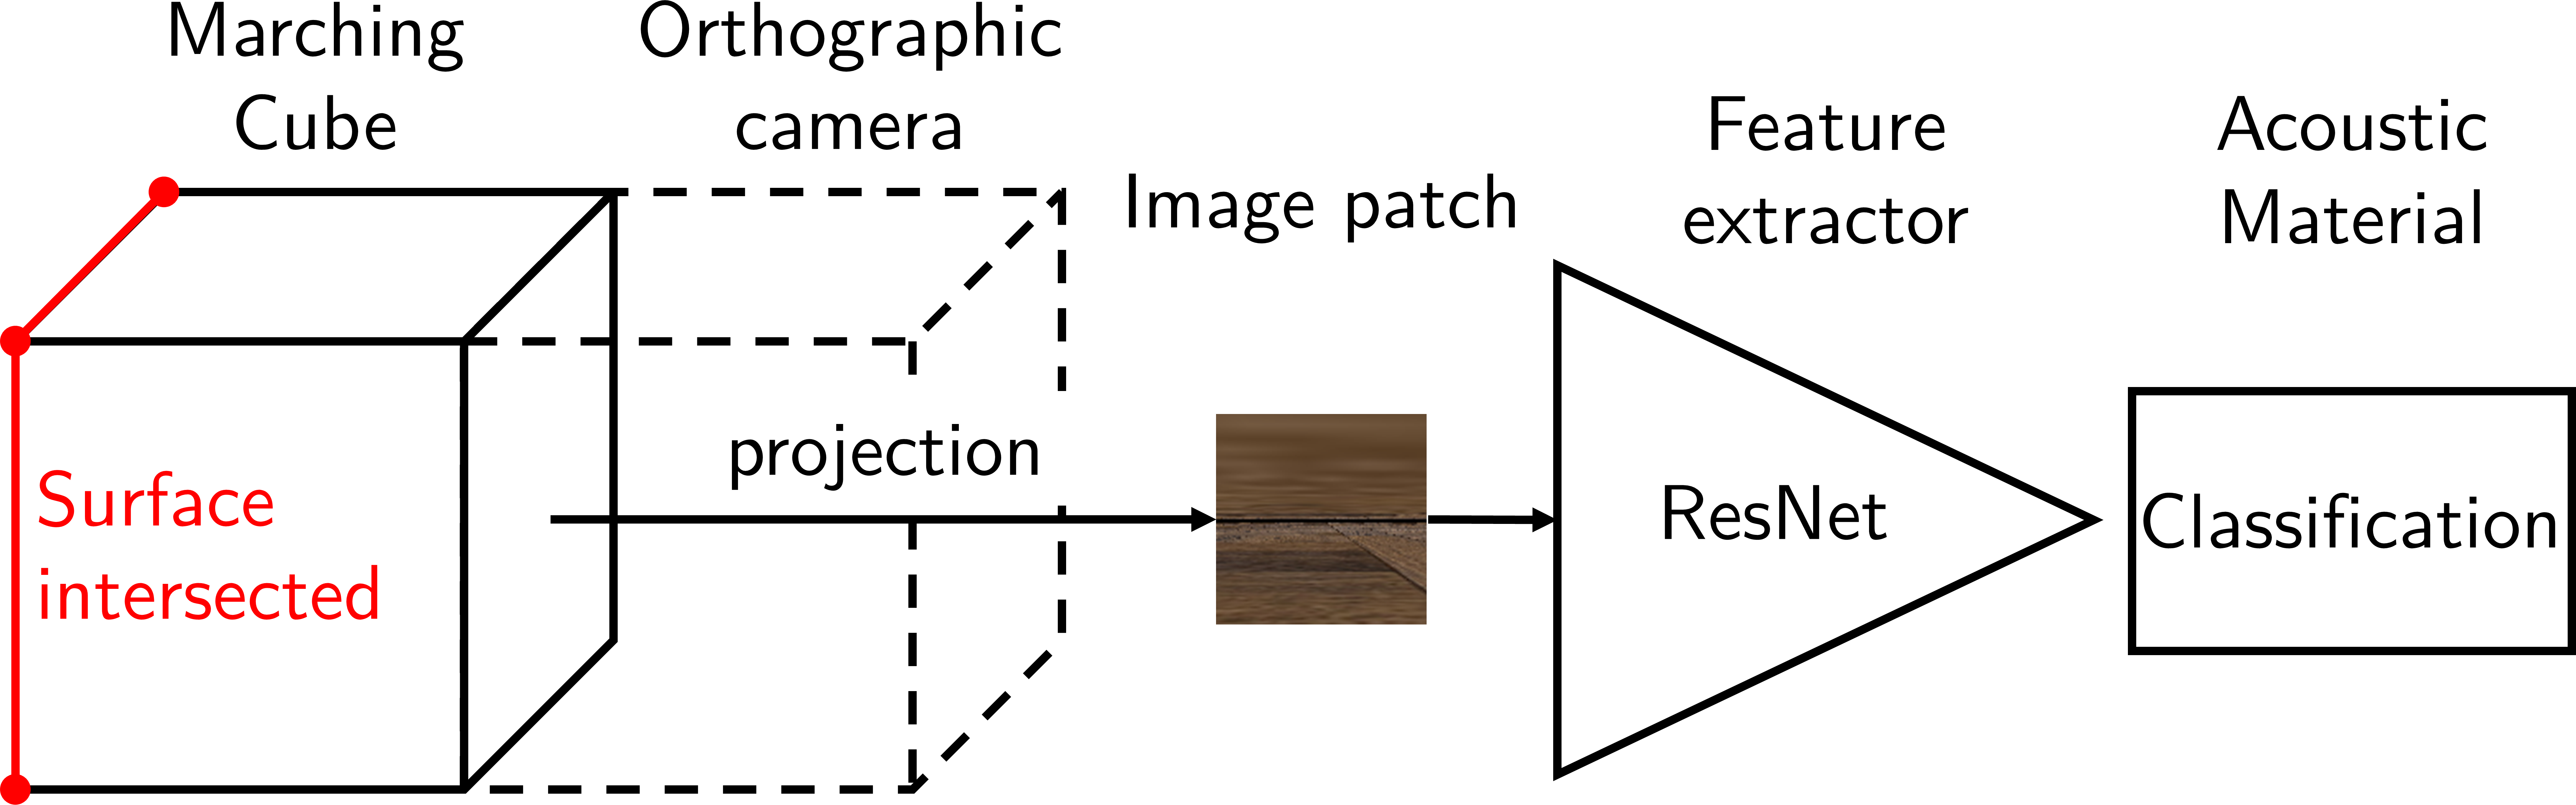
\includegraphics[width=1\columnwidth]{ism-patch_generation}
    \caption{Image patch generation: surfaces intersected by marching cubes are projected onto image patches with a camera by rasterising vertices via orthographic projections of the delimited portion of the surface. The resulting image patch is then fed to a neural network to extract features for semantic classification. Through a one-to-many mapping, semantics attributed to a patch, via embeddings classification, map to acoustic parameters.}
\label{fig:ism-patch_generation}
\end{figure}

\subsection{Camera Projection}
Image patches are generated whenever a marching cube intersects a surface by an entire side, i.e. four consecutive corners of each marching cube. An orthographic camera, positioned at the centre of the neighbouring cube, rasterises sub-surfaces delimited by the cube. The camera is positioned on the opposite side of the four intersected corners, facing the surface that is intersected; see Figure~\ref{fig:ism-patch_generation}. 
By using OpenGL rasterisation, surfaces are renderered orthographically from world space, defining the camera clipping space as the volume of the marching cube. Sampling image data from textures, the rasterisation stage produces an image patch representing the projection of the portion of the surface inscribed by a marching cube. Marching cubes intersecting in four consecutive corners ensure that the orthographic camera is perpendicular to the surface.\par

\subsection{Acoustic Material Classifier}
Image patches projected from marching cubes provide input to a neural network, a ResNet50 \citep{he2016deep} backbone that operates as a feature extractor, whose output is forwarded to a densely connected layer. This last layer classifies predicted embeddings into acoustic material categories. The network was trained on the OpenSurfaces dataset \citep{bell2013opensurfaces}, learning mappings between visual appearances of surfaces from 34 material classes and semantic labels, as described in Chapter~\ref{ch:Materials}. The network, pre-trained on ImageNet \citep{deng2009imagenet}, learns on $32\times32$ pixel resolution image patches that are extracted from appearances sampled from OpenSurfaces, assembling a dataset of about 13M images, split into 9M and 4M train and evaluation sets, respectively. Via a one-to-many mapping, 34 categories from the OpenSurfaces dataset map to acoustic materials, and, given 11 acoustic materials, subdividing into two levels of mass density, the visual labels are mapped to 22 acoustic materials.\par

\subsection{Frequency-Dependent Reverb Approximation}
The ISM estimates attenuation functions for a given listener position, with respect to a source in space, drawing from Habet's implementation~\citep{habets2006room} to estimate $h$ reverb response functions based on the spatial $[x, y, z]$ coordinates of a sound source, $\mathbf{s}$, a listener, $\mathbf{l}$, at each time step $t$ as 
\begin{equation}
\label{eq:ism-base}
h(\mathbf{l}, \mathbf{s}, t) = \sum_{\mathbf{p} \in \pazocal{P}} \sum_{\mathbf{m} \in \pazocal{M}} \beta_{-x}^{|\mathit{m_x - q}|} \beta_{+x}^{|\mathit{m_x}|} \beta_{-y}^{|\mathit{m_y - j}|} \beta_{+y}^{|\mathit{m_y}|} \beta_{-z}^{|\mathit{m_z - k}|}  \beta_{+z}^{|\mathit{m_z}|} \frac{\delta(t - \tau)}{4\pi \mathit{d}}\textrm{.}
\end{equation}
Here, $\pazocal{M} = \{(m_x, m_y, m_z): -N \leq m_x, m_y, m_z \leq +N\}$ determines the number of points per dimension based on the size of the input acoustic volume and the timestep, dependent on the desired sampling frequency, on the length of the output RIR, and the order of reflections $N$. $\pazocal{P} = \{ (q, j, k): q, j, k \in {0, 1} \}$ determines possible combinations of image sources mirrored in the three dimensions from every boundary in the acoustic volume to consider higher-order reflections, which are computed by $\delta (t - \tau)$, where $\tau = \frac{||\mathbf{R_p} + \mathbf{R_m}||}{c}$ indicates the reflection time delay by dividing the measured distance between mirrored image positions $\mathbf{R_p} + \mathbf{R_m}$ and the listener by the speed of sound $c$, $d$ is the distance term and is calculated as $\sqrt{(\mathbf{R_m}+\mathbf{R_p})}^2$. With combinations in $\pazocal{P}$, image positions are determined by
\begin{align*}
&\mathbf{R_p} = [ (1 - 2q)\mathbf{s_x} - \mathbf{l_x}, (1 - 2j)\mathbf{s_y} - \mathbf{l_y}, (1 - 2k)\mathbf{s_z} - \mathbf{l_z} ] 
\quad \textrm{and} \\
&\mathbf{R_m} = [2 m_x l_x, 2 m_y l_y, 2 m_z l_z]\textrm{.}
\end{align*}
The ISM computes multiple $h$ functions across frequency-dependent reflection coefficients, increasing the accuracy of simulated reflections from boundaries of the acoustic volume. In Equation~\ref{eq:ism-base}, $\beta$ reflection coefficients determine the energy attenuation of a computed reflection, specifying a single reflection coefficient mapping to each side of the acoustic volume; namely, $-x$ to $+z$  (left, right, top, bottom, front and back side). As these coefficients imply that materials apply a constant attenuation over the frequency spectrum, they can be redefined as $\beta_{-x,f}, \beta_{+x,f},~\dots, ~\beta_{+z,f}~\forall f \in \pazocal{F}: \{125, 250, 500, 1000, 2000, 4000\} Hz$, where $f$ indicates the frequency bin mapping to a reflection coefficient, adding a further dimension to Equation~\ref{eq:ism-base}, which can be defined as:
\begin{equation}\label{eq:fd-ism}    
 h(\mathbf{l}, \mathbf{s}, f, t) = \sum_{\mathbf{p} \in \pazocal{P}} \sum_{\mathbf{m} \in \pazocal{M}} \sum_{f \in \pazocal{F}}\cdot
\beta_{ {-x,f } }^{|\mathit{m_x - q}|} \beta_{+x, f }^{|\mathit{m_x}|} \beta_{ -y,f}^{|\mathit{m_y - j}|} \beta_{ +y, f }^{|\mathit{m_y}|} \beta_{ -z, f }^{|\mathit{m_z - k}|} \beta_{ +z, f }^{|\mathit{m_z}|} \frac{\delta(t - \tau)}{4\pi \mathit{d}}
\end{equation}
Frequency-dependent reflection coefficients enable the mapping between boundaries in the environment and acoustic materials. Equation~\ref{eq:fd-ism} produces separate $h$ attenuation functions for frequency bins in $\pazocal{F}$, associated to the common six octave bands defined by the acoustic materials to cover the equivalent rectangular bandwidth-number scale \citep{kuttruff2016room, savioja2015overview}.

\subsection{Audio Rendering}
The generated frequency-dependent $h$ functions can be treated as finite impulse responses and can be used to produce a broadband RIR. Filters based around frequency-dependent absorption coefficients (six in this case) can generate a new set of $h$ functions that contribute to a specific band of the equivalent rectangular bandwidth scale. Phase-invariant low-pass filters based on \citep{smith1997scientist}'s designs are combined with their corresponding frequency-inverted counterparts that we chain to produce band-pass filters. Filters are complementary to each other in the frequency domain ($20Hz$ to $20kHz$), summing to a flat magnitude response. Processed $h$ functions are then summed into a resulting RIR, which we convolve to anechoic audio to propagate audio in the simulated acoustic environment. \par

\subsection{Acoustic Volume Absorption}
This ISM adapts to non-enclosed or partially enclosed space by determining acoustic materials associated with the six sides of the cuboid acoustic volume: when no image patches are assigned to a given side, its respective reflections are ignored, i.e. maximum attenuation. Otherwise, let $\mathbf{M}_{-x~\dots~+z} = \{ \alpha_{0, f}, \alpha_{1, f},~\dots~, \alpha_{n, f} \}$ be the vectors of acoustic materials corresponding to marching cubes, describing frequency-dependent $\alpha$ acoustic absorption. Considering marching cubes intersecting surfaces associated with a side of the volume at $n$ points, acoustic materials generated by the \emph{material recognition} stage substitute elements of vector $\mathbf{M}$, while the remaining elements default to air absorption \cite{kates2020adding}. Acoustic materials contribute to a final set of acoustic absorption coefficients $\alpha_{-x,f}, \alpha_{+x,f},~\dots~\alpha_{+z,f}$ equivalent, as $\beta = \sqrt{1 - \alpha}$ \cite{allen1979image}, to the reflection coefficients considered in Equation~\ref{eq:fd-ism}. The contribution of each acoustic material is weighted based on the number of image patches found for each side and the total number of possible image patches $P^3$ that can be associated with each side, dependent on the resolution of the \emph{geometry reduction} stage. Hence, the weighted average determining acoustic absorption for each side of the acoustic volume can be defined as: 
\begin{equation}
    \alpha_{-x,f}, \alpha_{+x,f},~\dots,~\alpha_{+z,f} = \frac{ \sum_{i=1}^{P^3} w_i~\mathbf{M}_{-x,i}, \mathbf{M}_{+x,i},~\dots,~\mathbf{M}_{+z,i} }{ \sum_{i = 1}^{P^3} w_i},
\label{eq:weighted_average}
\end{equation}
where $w$ indicates the weights vector defining acoustic material contribution: 
\begin{equation}
    w_i = \begin{cases}
        \frac{n}{P^3}& \text{if}~i \leq n \\
        \frac{(P^3 - n)}{P^3}& \text{otherwise}
    \end{cases}
\label{eq:patch_contribution}
\end{equation}
Hence, the contribution of acoustic materials to the ISM volume depends on the surface intersected by marching cubes.

\section{Preliminary ISM Evaluation}

\subsection{Objective Evaluation}
A preliminary objective evaluation was conducted on the initial renderer prototype by deploying the proposed pipeline on a set of scenes, providing coverage of a wide range of practical use cases: ``Room'', ``Office'', ``Church'' and ``Village''. These have increasing volume as reported in Table~\ref{tab:ism_scene_scores}. ``Room'' is a real conference room captured using a LiDAR scanner, FARO Focus\textsuperscript{3D} X300. The remaining scenes are virtual environments that are common in game development. \par
Using the initial ISM prototype renderer, RIRs are generated across the four scenes, applying all stages of our pipeline as offline procedures, comparing acoustic simulations with inferred acoustic materials to simulations with manually tagged materials. These acoustic simulations assume omnidirectional sources and receivers, as no human listeners are involved in the comparison. Hence, simulations disregard directivity patterns or head-related acoustic phenomena. Source-receiver position pairs are consistent across RIRs pairs. Objective metrics associated with room acoustic parameters are extracted to compare the output of each acoustic simulation.\par

\subsection{Subjective Evaluation}
\subsubsection{Overview}
To gather insights on the potential deployment of the pipeline on auralisation systems for interactive applications, a preliminary evaluation tests the proposed system on a set of scenes, where features of audio transmissions between a source and a listener are extracted to gain insights into the visual-acoustic matching performance offered by the initial design of the renderer. \par

\subsubsection{Procedure}
The preliminary subjective evaluation procedure uses the prototype renderer to construct a cuboid acoustic volume encapsulating the source-listener pair, producing image patches with captured surfaces and infering acoustic materials to generate acoustic materials associated with the volume. For each scene, \emph{two} RIRs are generated to allow auralisations: \emph{one} using automatically-generated acoustic materials and \emph{one} using manually-tagged acoustic materials. RIRs are compared by utilising a pre-trained network for subjective comparison between auralisations produced via convolution of RIRs to audio from a database of anechoic recordings of sound events from the TUT Sound Event database \citep{sharath_adavanne_2018_1237752}. The deep audio perceptual similarity metric, CDPAM \citep{manocha2021cdpam}, trained on a dataset of human judgements, expresses distances between two audio signals and a reference. The network can be adopted as a metric that measures the Just Noticeable Difference (JND) as a distance $D(x_{per}, x_{ref})$ between a reference signal $x_{ref}$ and a perturbed $x_{per}$. Reverberation or equalisation are among the perturbation factors affecting the measured distance. Perceptual distance scores greater than $1$ indicate that a human would distinguish them as distinct. The objective of the evaluation is to evaluate whether sound propagated using the rendering pipeline with inferred acoustic materials is perceptually indistinguishable from sound propagated with manually tagged materials. RIRs are used to generate convolutions of a collection $S$ of 2700 audio samples to determine the perceptual distances $D(x_{predicted, i},~x_{tagged, i})~\forall i \in S~$ between convolutions using predicted and manually tagged materials.\par

\subsection{Results}
The classifier takes an average of $0.03s$ to infer the acoustic material from an image. The prototype rendering pipeline is tested by comparing acoustic energy decay across computed RIRs, as it expresses reflection paths computed on scene geometry for a given source-listener position pair. We extract metrics from impulse responses following \cite{lima_RIR_Parameters}'s feature analysis definitions. By fitting energy decay curves, the $T_{60}$ reverberation metric, the $C_{50}$ clarity index, and the $D_{50}$ definition index are determined. $C_{50}$ and $D_{50}$ indices are dependent upon the ratio between the power of early and late reflections. See Table~\ref{tab:ism_scene_scores} for estimated reverberation, clarity and definition scores across scenes. Figure~\ref{fig:ism_perceptual_evaluation} shows distributions of perceptual distances from RIRs generated using automatically tagged materials to RIRs generated with manually assigned materials. \par


\begin{table*}
  \caption{Features extracted from room impulse response pairs generated using the proposed system and metrics of corresponding input environments. Each pair has a \emph{predicted} and \emph{tagged} RIR, referring to acoustic materials being inferred with acoustic material classification or tagged manually. $t$ refers to the time taken to compute reflections, and $P$ indicates the number of sampling points per dimension.}
  \label{tab:ism_scene_scores}
	\centering%
\begin{tabular}{lllll}
                         & Room             & Office            & Church         & Village        \\ \midrule
Scene                    & 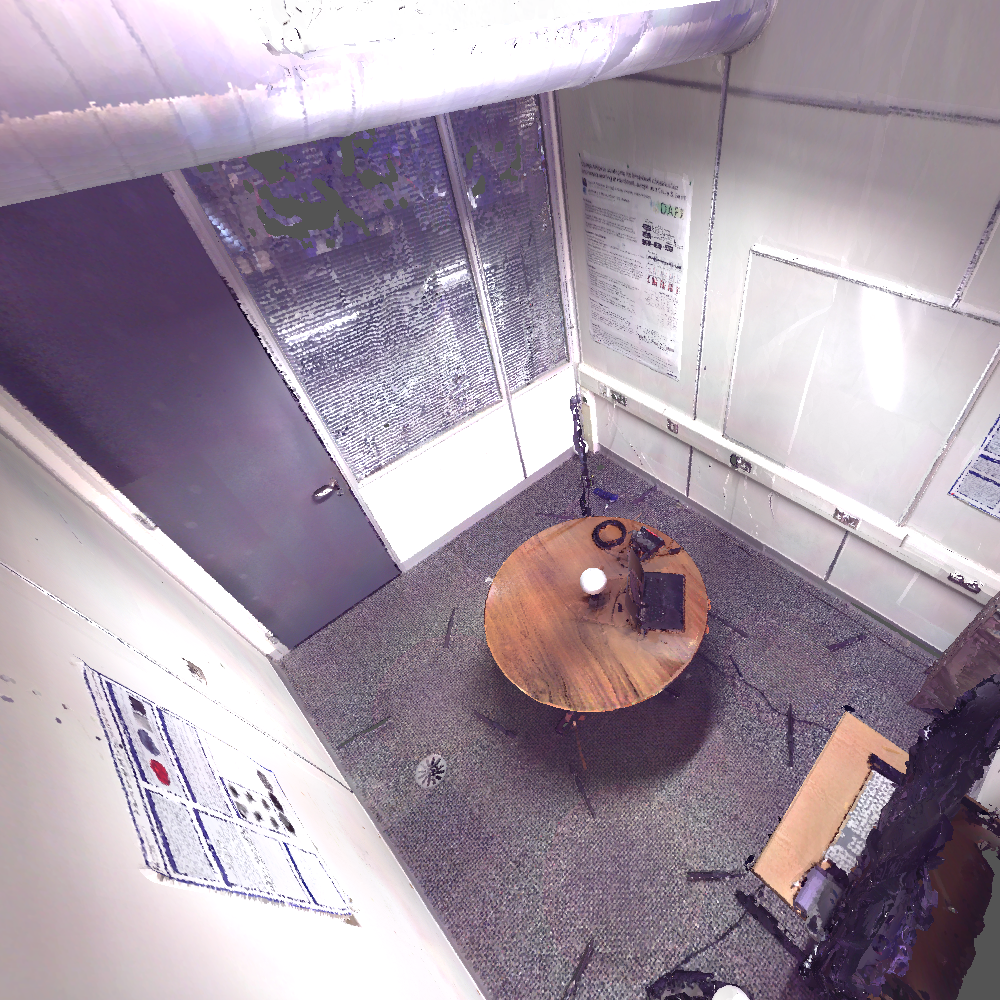
\includegraphics[width=0.16\textwidth]{Room}  & 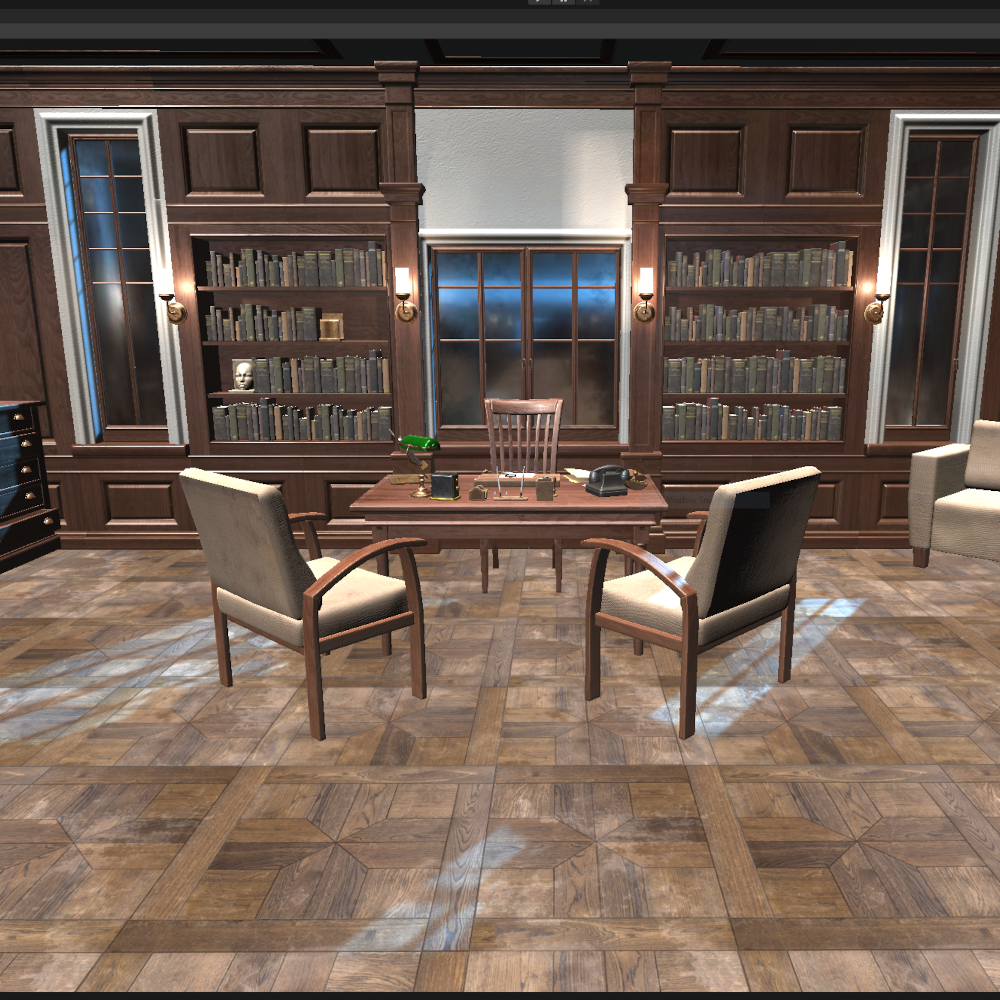
\includegraphics[width=0.16\textwidth]{Office} & 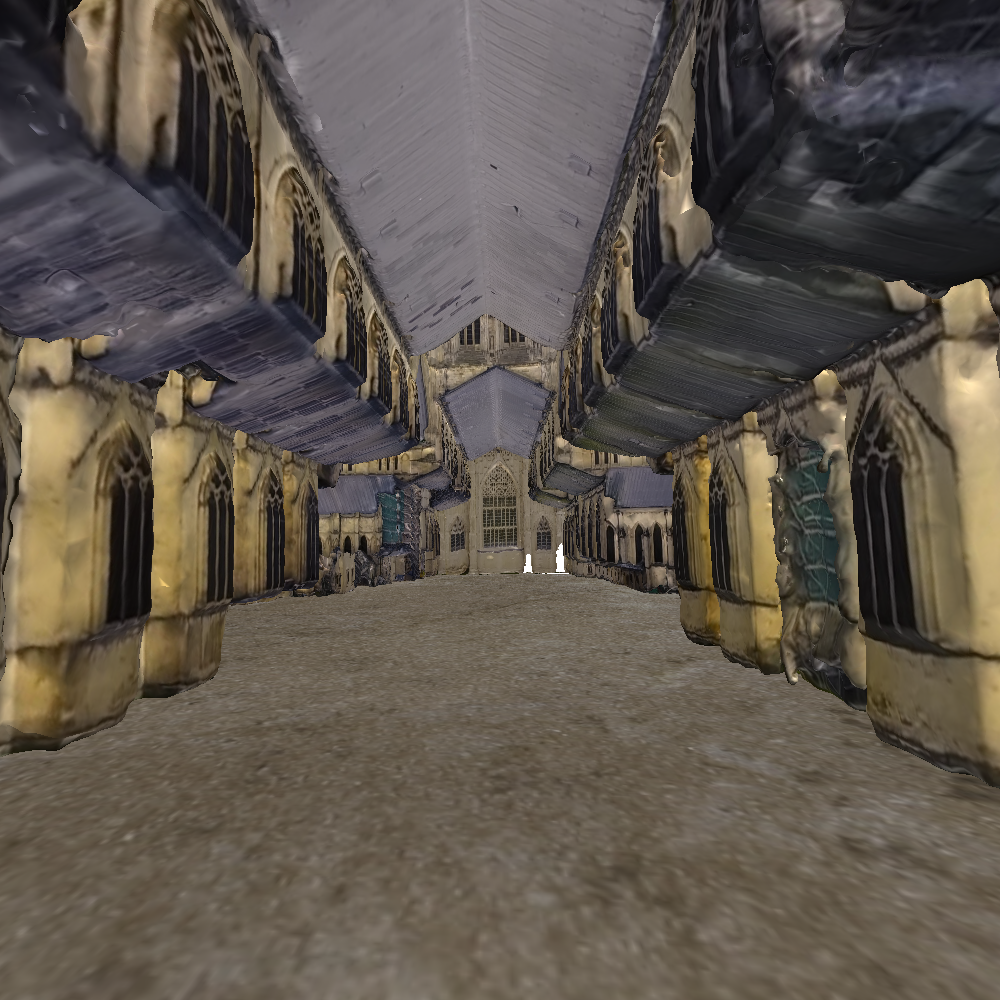
\includegraphics[width=0.16\textwidth]{Church} & 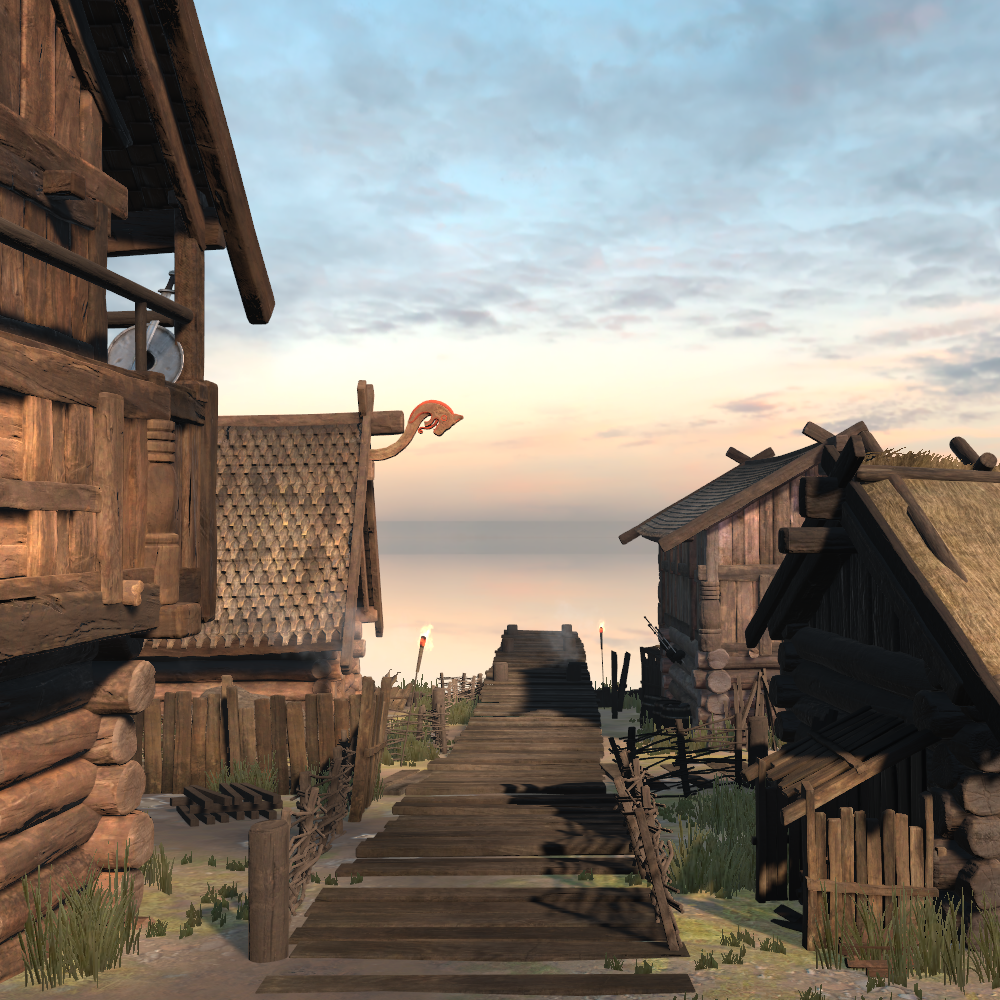
\includegraphics[width=0.16\textwidth]{Village} \\
Acoustic Volume          & 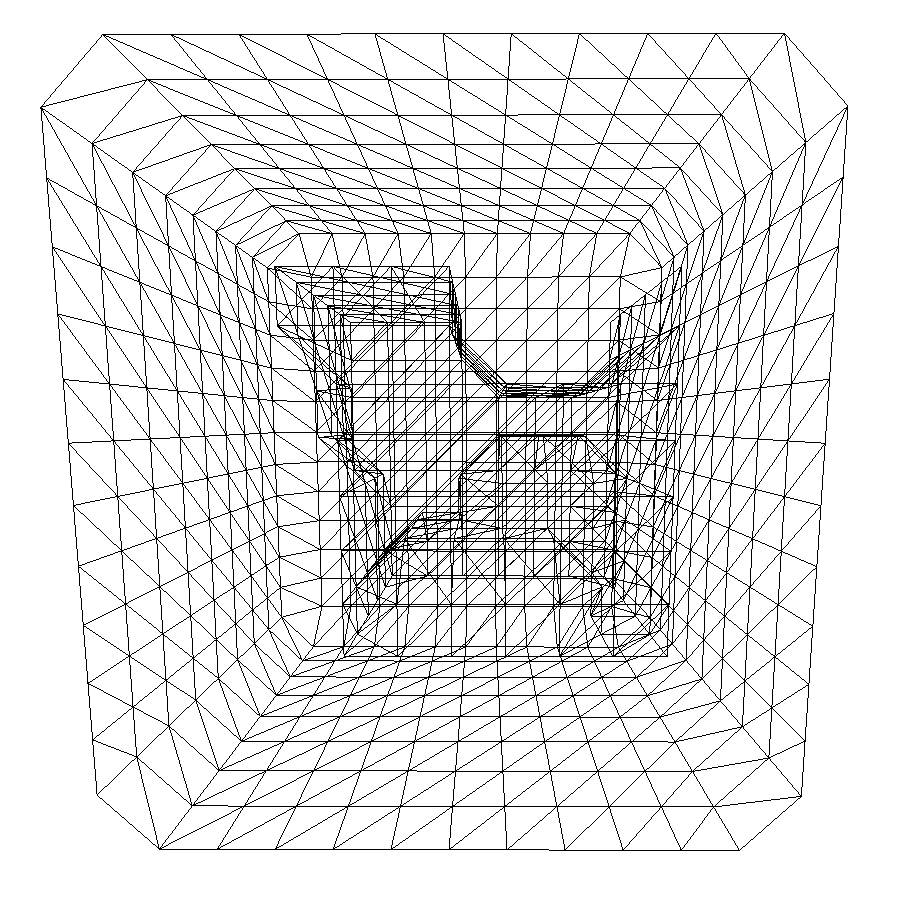
\includegraphics[width=0.16\textwidth]{Room_mc}  & 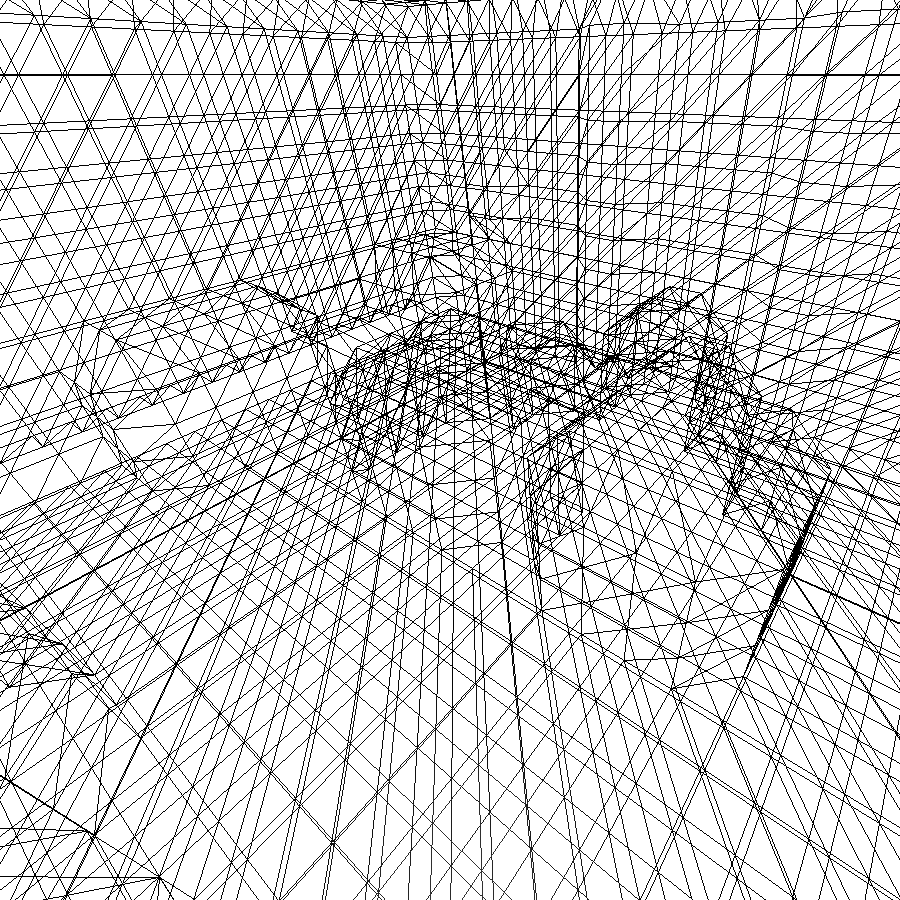
\includegraphics[width=0.16\textwidth]{Office_mc} & 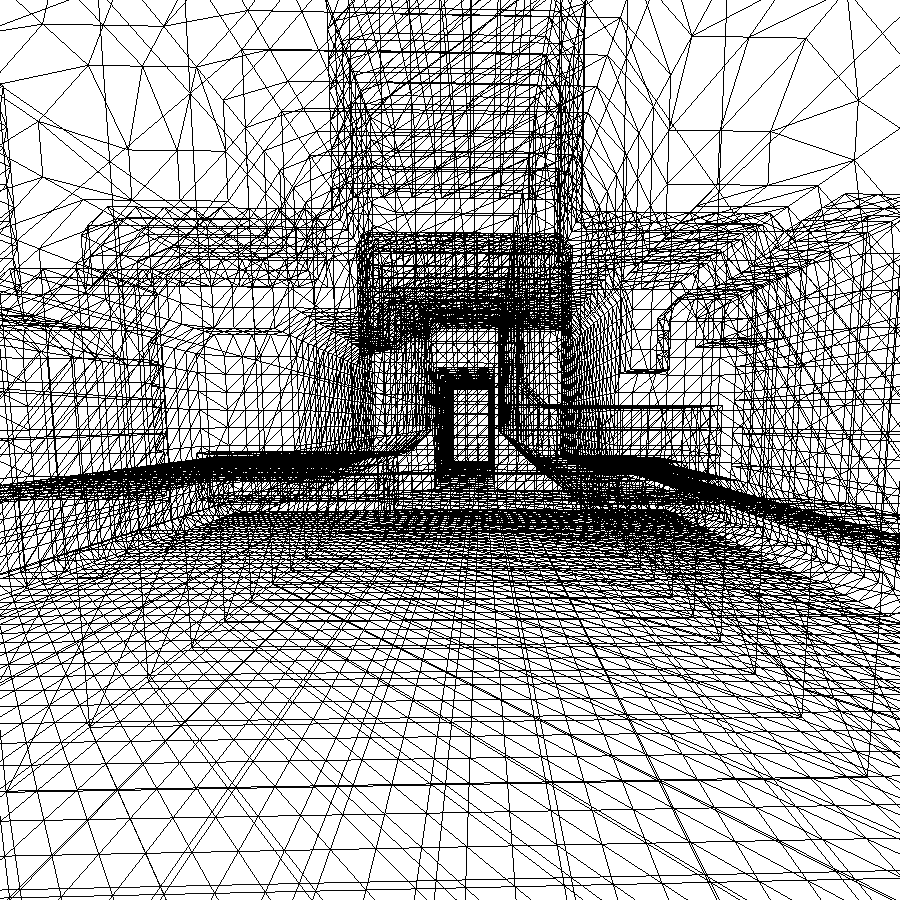
\includegraphics[width=0.16\textwidth]{Church_mc} & 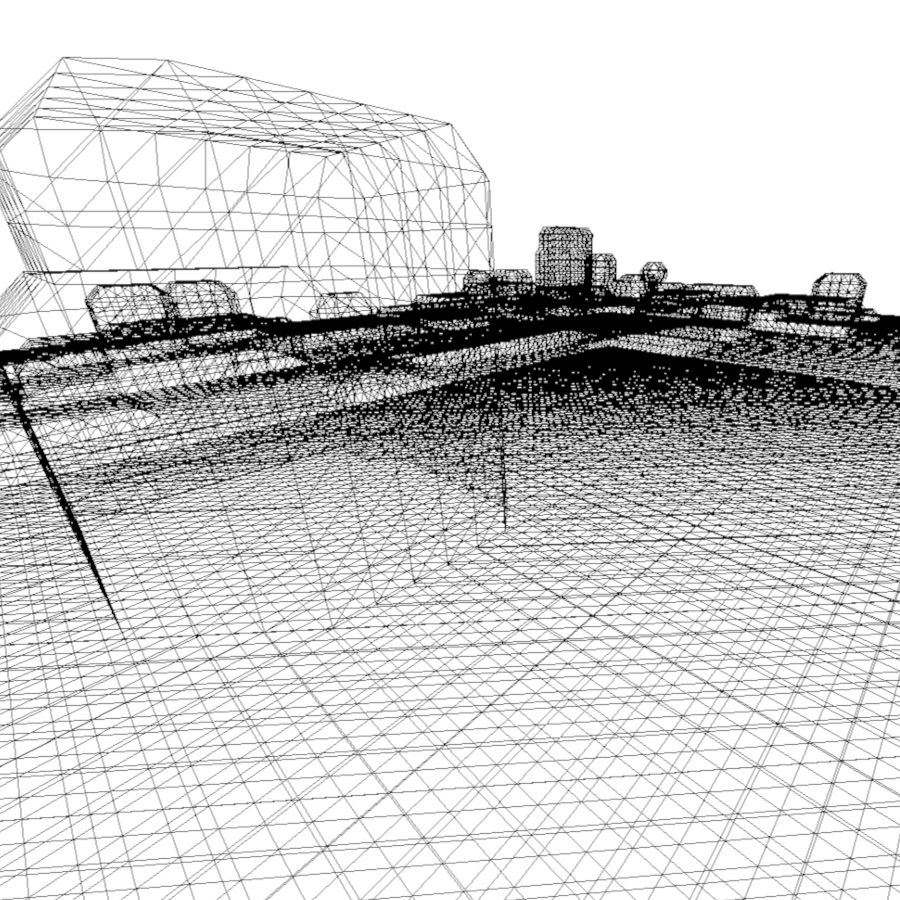
\includegraphics[width=0.16\textwidth]{Village_mc} \\ \midrule
Volume $(m^3)$           & $3.43 \times 10$      & $8.64 \times 10^3$     & $4.83 \times 10^4$  & $3.45 \times 10^8$  \\
Triangles                & 15.4M            & 0.973M            & 0.49M          & 9.6M           \\
P                        & $16^3$           & $32^3$            & $64^3$         & $128^3$        \\
Order                    & 3                & 4                 & 5              & 1              \\
$t (s) $                 & 2.824            & 3.53              & 2.791          & 1.25           \\ \midrule
predicted $T_{60} (s)$   & 0.997            & 1.705             & 5.982          & 0.103          \\
tagged $T_{60}(s)$       & 0.331            & 0.734             & 9.6            & 0.124          \\
$T_{60}$ error           & 0.666            & 0.971             & 3.618          & 0.021          \\ \midrule
predicted $C_{50}$       & 1.278            & -2.613            & -12.341        & -5.724         \\
tagged $C_{50}$          & 0.709            & -1.193            & -13.706        & -3.036         \\
$C_{50}$ error           & 0.569            & 1.42              & 1.365          & 2.688          \\ \midrule
predicted $D_{50}$       & 0.499            & 0.384             & 0.048          & 0.275          \\
tagged $D_{50}$          & 0.509            & 0.619             & 0.035          & 0.36          \\
$D_{50}$ error           & 0.01             & 0.235             & 0.013           & 0.085          \\
\end{tabular}%
\end{table*}

\begin{figure}[htbp]
    \centering
    \includegraphics[width=1\linewidth]{ism_scene_plots}
    \caption{Comparison between room impulse responses, generated using the proposed framework.\emph{Predicted} RIRs are produced using materials inferred by the automatic acoustic material classification, while the \emph{tagged} counterparts have manually tagged acoustic materials. Rows show scenes in ascending order of volume; Columns from left to right show a render of the scene with an overlapped polygonised acoustic volume resulting from the marching cubes algorithm; a time-domain visualisation of the impulse response using \emph{predicted} materials, followed by the counterpart with \emph{tagged} materials; finally, the last two columns show spectrograms of the two. RIR pairs are generated, maintaining the same positions of source and listener.}
    \label{fig:ism_scene_plots}
\end{figure}

\begin{figure}[htbp]
 \centering % avoid the use of \begin{center}...\end{center} and use \centering instead (more compact)
 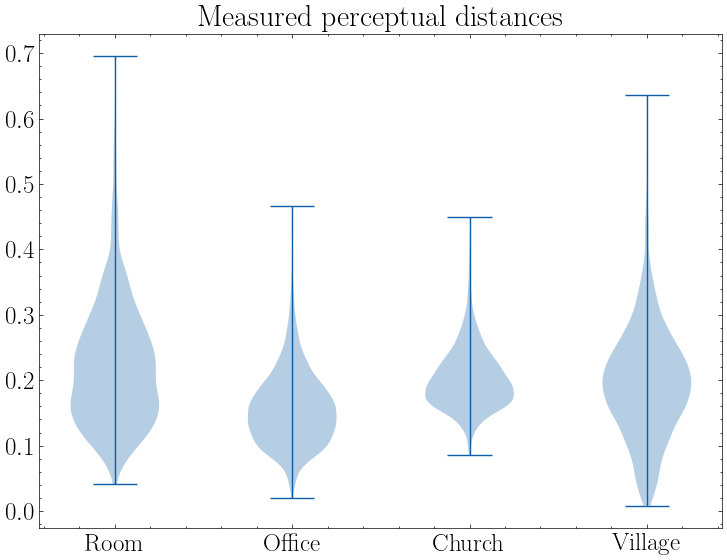
\includegraphics[width=1\linewidth]{ism_perceptual_distances}
 \caption{Distributions of perceptual distances between pairwise comparisons of audio recordings convolved to generated RIR pairs.
A collection of everyday sounds is propagated for each pair, producing convolution pairs. By employing a learned metric, the perceptual distance between RIR with \emph{predicted} and \emph{tagged} materials is measured. The violin plot reports that all distances fall below one just noticeable difference, indicating that a human would be unlikely to distinguish between the two convolutions.}
 \label{fig:ism_perceptual_evaluation}
\end{figure}

\subsection{Discussion}
\subsubsection{Overview}
Given that procedures of isosurface extraction and computation of frequency-dependent impulse responses run on CPU programs, the timings recorded across the four scenes with increasing spatial resolution suggest that the pipeline would be practical for interactive platforms. Especially when considering dynamic and incremented geometry typical of extended reality systems. Furthermore, GPU implementations of the ISM efficiently distribute sources across parallel workers, allowing for real-time RIR generation \citep{diaz2021gpurir}. The technique illustrates promise in the domain of streaming geometry, where virtual environments are constructed via spatial mapping services for visualisation on extended reality displays. \par
There is a necessity for understanding the acoustic information to be associated with this streamed mesh data. The nature of this approach facilitates mesh ingestion and updates to the binary field; subsequent subregions of the marching cube volume can be iteratively updated, and the resultant RIR to take stock of updated geometry can thus be generated. Despite overcoming the limitations of ISMs in propagating sound in non-enclosed environments, phenomena such as the occlusion of sound sources and arbitrary shapes of the environments are not considered. Occlusion and visibility of sound sources can be solved by combining the ISM with ray tracing, allowing for checking source visibility and introducing limited overhead thanks to their GPU implementations \citep{taylor2012guided}.\par

\subsubsection{Acoustic Material Approximation}
The complexity of the pipeline depends upon the nature of the complex scenes and the number of points in which surfaces are sampled. Considering the overhead introduced by the acoustic material classifier, the complexity of the pipeline scales linearly with the number of surface intersections in the environment. Hence, the worst complexity occurs when each marching cube intersects scene geometry. In addition, despite the classifier's reasonable accuracy on test data, no ablation studies have been conducted to reduce the architecture to a minimum topology and further optimise complexity. Acoustic materials associated with each side of the calculated volume contribute to a mean, causing the ISM to approximate the computation of specular reflections, neglecting characteristics of surfaces, such as position or orientation. This approximation can be overcome by eliminating the process of averaging acoustic materials and reformulating the computation of image sources defined in Equation~\ref{eq:fd-ism} to refer to individual acoustic materials mapped to the acoustic volume. However, the reformulation would affect the timestep of computed $h$ functions, constraining it to the geometry reduction resolution, resulting in an arbitrary scale that should be interpolated to the time scale. \par
The benefits of removing mean acoustic material would include the ability to simulate arbitrary shapes of surfaces by having acoustic materials mapped to marching cubes. This process would need to consider Nyquist sampling theory to determine the appropriate cube sizes to simulate accurate acoustics whilst maintaining specular plausibility in the frequencies simulated. \citep{pelzer2010frequency}'s work, in addition, suggests that the resolution of the geometry reduction process can be set according to perceptual responses in the resulting simulation. Their experiments reveal that geometry with small structural details can be excluded from acoustic modelling, maintaining the perceived quality, and this acts as a motivating basis for this future iterative study. \par

\subsubsection{Geometry Reduction}
Determining space subdivision through the resolution factor $P^3$ of the \emph{geometry reduction} stage has an effect on the volume reconstruction and generation of image patches, which directly map to acoustic materials. Larger resolutions require more marching cubes, causing the number of orthographic projections from surfaces to increase, resulting in a higher number of forward passes through the feature extractor, finally resulting in increased computational overhead. In order to maintain perceptual accuracy and produce plausible acoustic simulations whilst minimising the spatial resolution to optimise execution times, further work would require subjective evaluations to derive optimal spatial resolution across varying scene geometry. \par

\subsubsection{Objective Evaluation}
The most noticeable differences between renders with predicted and manually tagged materials are due to different decays of acoustic energy. By considering spectrograms of generated RIRs shown in Figure~\ref{fig:ism_scene_plots}, the different acoustic materials influence the decay of energy over time. As a result, there are errors relative to reverberation, definition and clarity; see Table~\ref{tab:ism_scene_scores}. \par

\subsection{Conclusions and Proposed Design Strategy}
The initial prototype represents a novel pipeline for acoustic rendering that is able to capture acoustic material characteristics of space around a listener using computer vision paradigms. These predicted acoustic material characteristics are used to generate input for sound propagation methods, producing plausible acoustic simulations. The proof-of-concept prototype is executed as offline procedures implemented as CPU programs, demonstrating the generation of RIRs that can be used in downstream convolution auralisations in real-time audio engines to propagate audio from virtual sound sources in simulated environments. The automated mapping between visual appearances and acoustic characteristics directly applies to extended reality platforms where the virtual environment is incrementally reconstructed as a listener explores their surroundings, enabling sound rendering to produce plausible acoustic simulations and removing human experts from the scene authoring process. \par
The preliminary design and evaluation cycle shows that the bottleneck of the rendering pipeline is at the core reverb approximation method, which should be improved by exploiting the space partitioning capabilities of the geometry reduction system. A ray tracer, for instance, may be a more suitable design choice to interact with individual partitions of the generated acoustic volume. \par

\section{Geometrical Acoustics Rendering Pipeline}\label{sec:ga-based-pipeline}
Considering the limiting factors of the ISM-based renderer, such as the inability to render complex architectures of environments or the inability to model acoustic phenomena beyond basic reverberation, the pipeline design was improved by adopting a ray tracer system. The targets for the rendering pipeline should be oriented towards: 
\begin{itemize}
    \item approximating basic acoustic phenomena based on architectural features of the environment where auditory interactions take place;
    \item enabling dynamic partitioning and indexing of the space, considering material recognition systems; 
    \item leveraging fast rendering and processing techniques that can be optimised for wearable computing platforms such as HMDs.
\end{itemize}


\subsubsection{Overview}
Ray tracing techniques have inherent limitations in modelling sound propagation within a space due to their nature of representing sound waves as rays. As discussed in Section~\ref{sec:bg-raytracing}, such limitations can cause physical inaccuracies in the simulated acoustic model, affecting the resulting audio interactions due to incorrectly simulated phenomena. An example is occlusion, where a sound source might be inaudible due to the obstruction and absence of paths between source and listener, though in the physical space, some low-frequency acoustic energy will still reach the listener due to their omnidirectional propagation patterns. \par
Although such limitations can cause inaccurate acoustic models, ray tracers still provide accurate reverberation and reflection approximations and are widely employed in modern acoustic surveying frameworks like ODEON\footnote{https://odeon.dk/} due to their ability to estimate key properties of soundfields and fast auralisations. Moreover, the constant rise in computing power offered by modern general-purpose GPUs offers fast implementations of geometrical acoustics that can be accelerated thanks to their architecture and the parallelisable nature of ray tracing \citep{savioja2010use}. \par

\subsection{Geometrical Search}
As discussed in Section~\ref{sec:bg-geometry-handling}, the foundations of an acoustic ray tracer lay in the interactions between the primitive used to approximate a propagating sound wave and the environment. The modelling of acoustic phenomena in acoustic simulations produced by ray tracers is a process dependent on physics interaction between the geometrical primitives that compose the complex scene. Ray Tracing uses rays and line segments as geometrical primitives, requiring the environment handling system to facilitate operations between rays and the complex scene.\par
The ray tracing-based renderer design implements a Bounding Volume Hierarchy (BVH) as a geometry handling system, allowing the dynamic indexing and searching of a given complex scene. The BVH implementation constructs a binary tree of AABBs encapsulating triangles of the mesh representing the VE and any entity interacting with the acoustic environment, e.g. a character representing a listener. 
A dynamic BVH implementation uses the environment, represented as a set of triangulated meshes, to construct a set of bounding boxes that facilitate geometrical search operations such as ray-box intersections or point-in-volume tests. \par
\begin{figure}[h]
    \centering
    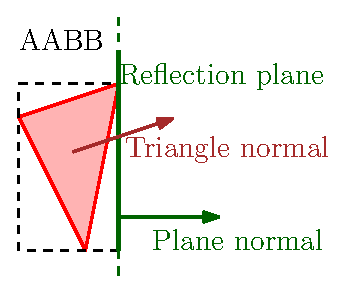
\includegraphics[width=0.4\linewidth]{aabb-normal}
    \caption{An Axis-Aligned Bounding Box (AABB), leaf node of a scene BVH, encapsulating a mesh triangle. The AABB facilitates geometry indexing and searching, optimising ray tracing operations such as ray-box intersections, and is used to provide reflection planes constructed based on the encapsulated triangle normal for reflecting rays.}
    \label{fig:aabb-normal}
\end{figure}

\subsection{Sound Propagation}
\begin{figure}
    \centering
    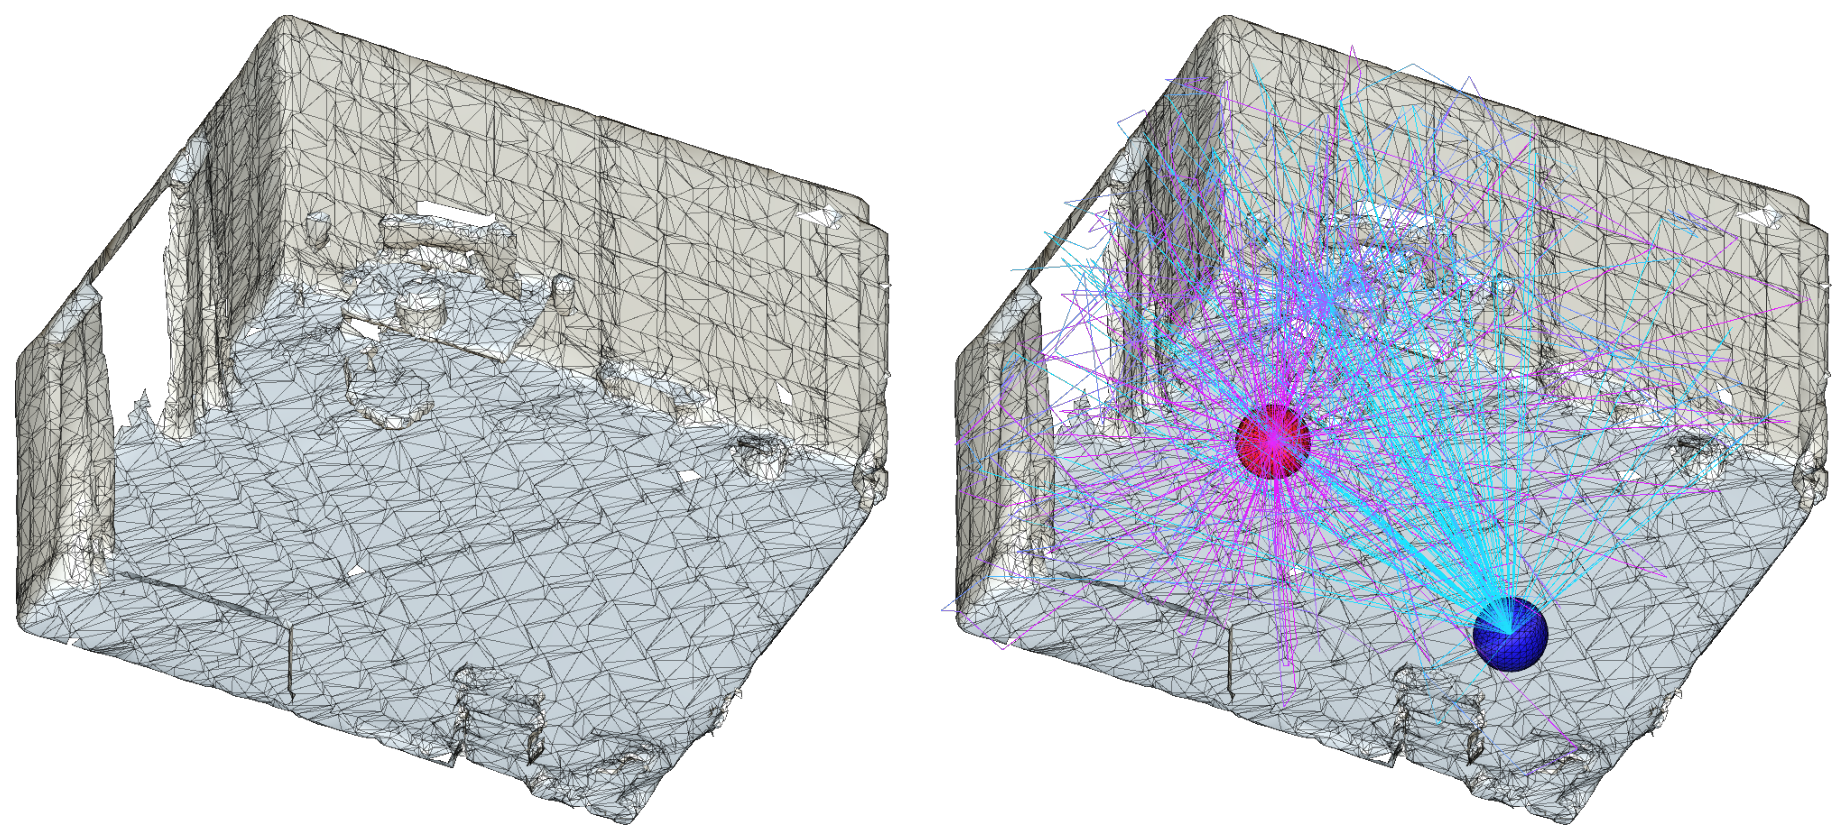
\includegraphics[width=1\linewidth]{rt-room-test}
    \caption{Visualisation of propagated rays from a sound source, red sphere, to a listener, blue sphere. The left image shows a visualisation of a triangulated mesh provided to the ray tracer; the right image shows rays originating from across uniformly distributed points on a sphere, reflecting off mesh triangles, and arriving at the listener sphere volume.}
    \label{fig:rt-room-demo}
\end{figure}
Rays propagate from a given spherical object, the sound source, visualised as a red sphere in Figure~\ref{fig:rt-room-demo}, originating from $N$ points uniformly distributed across the azimuth and elevation of the sphere. This chapter deals with the approximation of basic acoustic phenomena achieved by rendering pipelines and excludes directivity patterns for sources and receivers; hence, sources and listeners are omnidirectional emitters and monopole detectors unless explicitly defined otherwise. Propagation paths between source and receiver are expressed as three-dimensional segments determined by intersections caused by rays, containing acoustic features such as acoustic energy carried. The number of rays emitted from the source determines the initial energy $e_0$ of propagation paths, $e_0 = 1 / N$, where the sum of all propagation paths amounts to 1. \par
Algorithm~\ref{alg:rt-main} shows an overview of the main procedure of the ray tracer renderer. Starting from uniform sampling across azimuth and elevation points of the spherical volume of $S$, rays, defined by their origin and direction, are emitted from the spatial position of $S$ and oriented based on the sampled points across the sphere \citep{shirley2008realistic}; in Lines~\ref{alg:rt-main-spher} and \ref{alg:rt-main-cart} of Algorithm~\ref{alg:rt-main} directions are converted from polar to cartesian coordinates.\par


\begin{algorithm}
  \caption{Main procedure of the ray tracer: propagation paths are computed given Source/Listener bounds $S$ and $L$, a number or rays $N$ to propagate, and a max order $o$. for each propagation point on the emitter bounds, the geometry is searched for intersections a number of times depending on found intersections and the max order. These paths are registered if they intersect with the listener bound L.}\label{alg:rt-main}
  \begin{algorithmic}[1]
    \State{} \textbf{define} $Ray(origin,~direction)$
    \State{} \textbf{define} {$Vector3(x,y,z)$}
    \State{} \textbf{define} {$Path(e_0)$}\Comment{$e_0$: initial path energy}
    \Function{$SphericalToCartesian$}{$r, p, e$}\Comment{$r$: radius, $p$: polar angle, $e$: elevation angle}
        \State{} \textbf{return} $Vector3(r * \cos{e} * \cos{p}, r * \sin{e}, r* \cos{e} * \sin{p})$
    \EndFunction{}
    \Procedure{ComputePropagationPaths}{$S, L, N, o$}
      \State{} $e_0\gets 1 / N$
      % \State $ray \gets Ray(S.position,~L.position-S.position)$
      % \If{$SearchIntersection(ray)$}
      %   \If{Intersection is between S and L}
      %       \State $O \gets true$
      %   \Else
      %       \State register direct path
      %   \EndIf
      % \Else
      %   \State register direct path
      % \EndIf
      \ForAll{$i \in [0..\sqrt{N}] $}\Comment{Uniform sphere sampling: azimuthal steps}
        \ForAll{$j \in [0..\sqrt{N}$]}\Comment{Uniform sphere sampling: elevation steps}
          \State{} $dir_{spherical} \gets Vector3(S.radius,~i(2\pi/\sqrt{N}),~\pi/2-j(\pi/\sqrt{N}))$\label{alg:rt-main-spher}
          \State{} $dir_{cartesian} \gets SphericalToCartesian(dir_{spherical})$\label{alg:rt-main-cart}
          \State{} $path \gets new~Path(e_0)$
          \State{} $path.addRay(new~Ray(S.position, dir_{cartesian}))$
          
            \ForAll{$order \in [0..o]$}
                \If{$path.currentRay$ Intersects $Listener.bounds$ }
                    \State{} register specular path \Comment{occlusion between path and L is computed}
                    \State{} \textbf{break}
                \EndIf{}
              \If{$intersection$ between Geometry and $path.currentRay$}
              \State{} $reflection \gets$ reflect $path.currentRay$ with $intersection$
              \State{} $path.addRay(new~Ray(intersection,~reflection))$
              \State{} $path.substractEnergy(intersection.absorption)$
              \EndIf{}
              \EndFor{}
            \EndFor{}
        \EndFor{}

    \EndProcedure{}
  \end{algorithmic}
\end{algorithm}

\subsubsection{Reflection}
\begin{figure}[h]
    \centering
    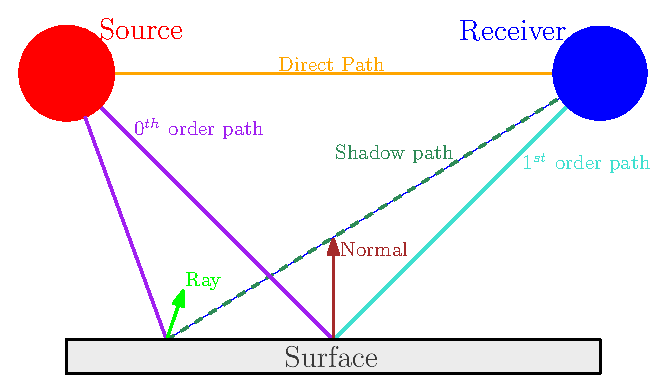
\includegraphics[width=1\linewidth]{rt-diagram}
    \caption{An overview of the implemented propagation path: paths are formed by segments found by searching intersections along rays originating from the Source. Depending on the reflection order allowed, see Algorithm~\ref{alg:rt-main}, rays can search for further intersections after reflecting around surface normals. Rays intersecting the Receiver will be registered as final propagation paths.}
\label{fig:rt-reflection-diagram}
\end{figure}
Figure~\ref{fig:rt-reflection-diagram} illustrates the computation of propagation paths overview in Algorithm~\ref{alg:rt-main}. For the sake of simplicity, only reflection paths are illustrated in the pseudocode listing, as shadow paths follow the same logic and registration procedure. The algorithm checks for intersection along rays propagating from the Source object bounds (the red sphere volume in Figure~\ref{fig:rt-room-demo}). Intersections found at surfaces create reflections around the computed surface normal by considering the leaf node AABBs encapsulating mesh triangles: rays are checked for collisions by traversing nodes of the scene BVH and testing ray-box collisions until a leaf node is reached. Leaf nodes are AABBs encapsulating mesh triangles; they are the primitives of the reconstructed acoustic volume. As shown in Figure~\ref{fig:aabb-normal}, propagation paths reflect around normals of reflections planes fit on surfaces of the AABB. Upon intersection of a ray with a leaf AABBs, the dot product of the encapsulated triangle normal is pre-computed for all six faces of the box; a plane is then fit on the face that aligns the most with the triangle normal, approximating the acoustic geometry to a Manhattan space.\par

\subsubsection{Absorption}
Leaf nodes of the scene BVH carry frequency-dependent acoustic absorption coefficients that affect the energy of propagation paths colliding with scene geometry. As discussed in Section~\ref{sec:mat-method}, coefficients express acoustic energy absorption over six frequency bands distributed over the human hearing frequency range. Propagation paths have $e_0$ initial energy across these six frequency bands, and upon collision with scene geometry, energy is absorbed based on the acoustic material assigned to the mesh triangle encapsulated in the colliding scene BVH leaf node. In pseudocode, $path.currentEnergy_f = path.currentEnergy * (1 - reflector.absorption_f)$ shows energy subtraction upon collision, with $f$ denoting frequency bands $\{ 125, 250, 500, 1000, 2000, 4000 \} Hz$ Table~\ref{tab:absorption-coeffs} shows example acoustic materials that can be attributed to leaf nodes. \par

\subsubsection{Shadow Paths}
Diffraction simulations, as demonstrated by diffraction modelling using the Uniform Theory of Diffraction (UTD) \cite{tsingos2001modeling}, use reflecting geometry and edges as sources of new diffracted rays, complementing specular reflections. Similarly, the ray tracer considers the possible connections between intersections at intermediate nodes of propagation paths and the receiver volume, see Figure~\ref{fig:rt-reflection-diagram}. Such shadow paths contribute to the modelling of the energy decay and exploit computations involved in geometry searches and occlusion tests. \par

\subsection{Energy Decay Modelling}
Due to frequency-dependent absorption properties of the scene geometry, specular and shadow rays generate propagation paths having varying remaining energy across the six frequency bands. Upon the execution of the procedure in Algorithm~\ref{alg:rt-main}, energy data can be extracted at the detector bounds by measuring all registered paths, creating frequency-dependent impulse responses, see Figure~\ref{fig:rir-freqdep-poisson}. To mitigate the deterministic nature of a ray tracer, a Poisson distribution can introduce randomness in the generation of an RIR, simulating chaotic aspects of acoustic energy reflected in an environment. \par
As~\cite{schroder2011physically}'s work demonstrates the efficacy of Monte Carlo methods combined with deterministic geometrical acoustics for physically-based acoustic rendering, the energy detected $E_f$ is used to control the reflection magnitude using Poisson distributions across the six frequency bands $f$. A time-varying Poisson distribution of Dirac-Delta pulses is generated, shown in Figure~\ref{fig:poisson-sequence}. The distribution models how, given a hypothetical environment with an emitter and detector, reflections would land at the detector over time: the transition from the direct signal and early reflections to late reflections is expressed as the density of detected reflections increased over time. \par
Following~\cite{schroder2011physically}'s model, the probability of the occurrence of reflections $w_n(\Delta t)$ within a time interval $\Delta t$ can be determined as:
\begin{equation}
\label{eq:poisson-distributed-diracs}
    w_n(\Delta t) = \frac{(\mu \Delta t)^n}{n!} e^{-\mu \Delta t} \quad n \in \mathbb{N}_0\textrm{,} \quad \mu > 0\textrm{,} \quad \Delta t \ge 0\textrm{,}
\end{equation}
where $\mu$ is the mean reflection occurrence. The interval can be determined as a function of a random number $z$ sampled from a uniform distribution: 
\begin{equation}
    \Delta t(z) = \frac{1}{\mu}ln(\frac{1}{z}) \quad 0 < z <= 1\textrm{,}
\end{equation}
with $\mu$ and the starting time $t_0$ dependent on the size of the environment $V$, determined by the root node of the scene BVH: 
\begin{equation}
    \mu = \frac{4\pi c^3 t^2}{V}\textrm{,} \quad t_0 = \sqrt[3]{\frac{2Vln2}{4\pi c^3}}\textrm{.}
\end{equation}

\begin{figure}[htbp]
    \centering
    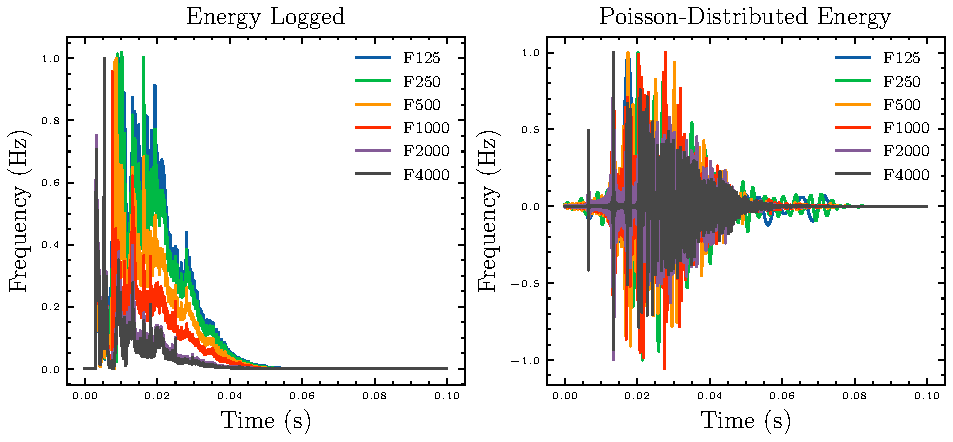
\includegraphics[width=1\linewidth]{rir-processing}
    \caption{Visualisation of frequency-dependent RIRs, represented as energy logging resulting from generated propagation paths for a given source-receiver computation of Algorithm~\ref{alg:rt-main}. Poisson distribution calculated based on the environment dimensions obtained from the generated BVH are then used to generate bipolar impulse responses.}
    \label{fig:rir-freqdep-poisson}
\end{figure}

\subsection{Impulse Response Construction}
\begin{figure}[htbp]
    \centering
    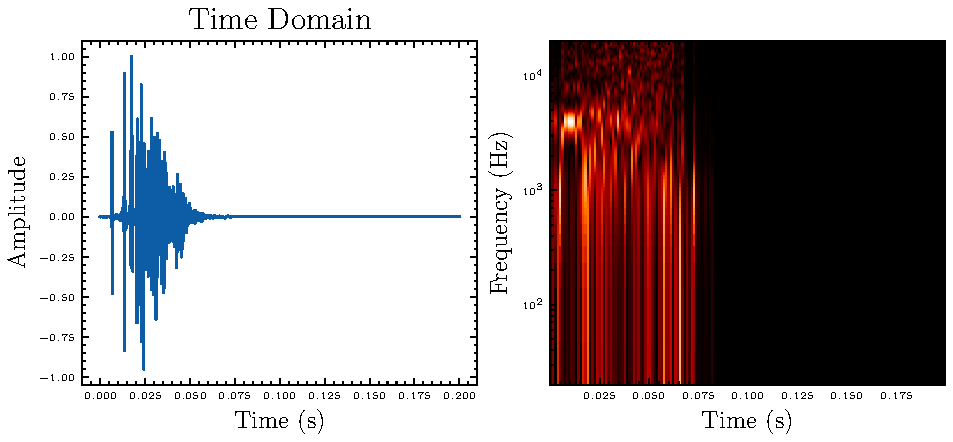
\includegraphics[width=1\linewidth]{rir-rt-final}
    \caption{Time and frequency-domain representations left and right subfigures, respectively, of frequency-dependent RIRs combined into a broadband monoaural response. }
    \label{fig:rir-freqdep-monoaural}
\end{figure}

\begin{figure}[htbp]
    \centering
    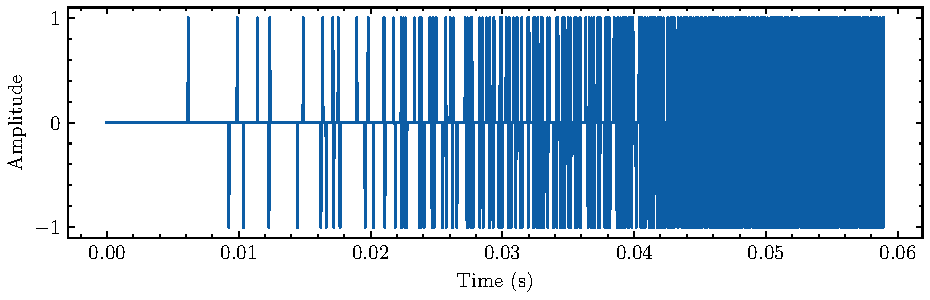
\includegraphics[width=1\linewidth]{poisson-sequence}
    \caption{A Poisson Distributions of Dirac-Delta functions generated for an environment with an approximate volume of $60m^3$. The distribution represents, using unit pulses, the time-dependent likelihood of reflections registered at a hypothetical receiver from a hypothetical source within an environment of said volume. Considered a stochastic model, the distribution is used to generate a synthetic RIR from energy logged by a ray tracer.}
    \label{fig:poisson-sequence}
\end{figure}

\begin{figure}[htbp]
    \centering
    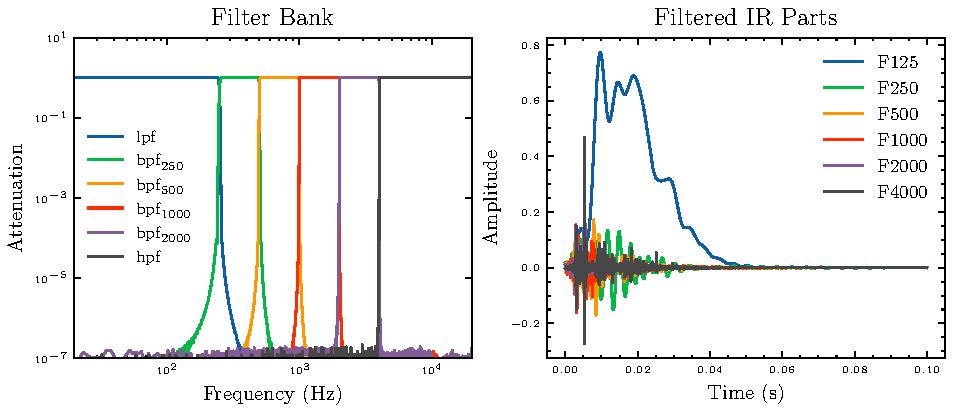
\includegraphics[width=1\linewidth]{filterbank}
    \caption{A filter bank partitioning the hearing range into octave bands associated with frequency-dependent energy logged by the geometrical acoustics renderer. The monoaural broadband IR visualised in Figure~\ref{fig:rir-freqdep-poisson} is constructed by having each frequency band filtered and contributing to its specific region. }
    \label{fig:filterbank}
\end{figure}
Using Dirac-Delta pulses to represent reflections, six sequences are generated with Equation~\ref{eq:poisson-distributed-diracs}, obtaining distributions similar to Figure~\ref{fig:poisson-sequence} for each frequency band $f$. The magnitude of these Poisson sequences $w_{n,f}$ follows the energy decay computed by the ray tracer: 
\begin{equation}
    h_f(t) = E_f(t)w_{n,f}(t)\textrm{,}
\end{equation}
determining frequency-dependent $h$ functions that can construct a monoaural RIR by filtering each frequency component $h_f$ and summing their aggregate to a broadband response. A filter bank determines the contribution of each $h_f$ towards its specific portion of the spectrum, dictated by the spectrum partitioning of the absorption coefficients used; it is composed of Finite Impulse Response (FIR) filters applied to the sequences. The filter bank is constructed using low-pass window-sinc filters for efficient computation against attenuation factors. High and band-pass filters are obtained via spectral inversions of window-sinc low-pass filters. Using \cite{smith1997scientist}'s implementation, the $h$ function is calculated for a low-pass $lpf$ filter for a digital sequence of $M$ points with sampling frequency $F_s$:
\begin{equation}
    lpf(i) = \frac{sin(2\pi f_c i)}{i\pi} \textrm{,}
\end{equation}
where $f_c$ indicates the cut-off frequency relative to $F_s$. Filters are computed over $M = 2^{14}$ points, obtaining over 120dB of stop-band attenuation, see Figure~\ref{fig:filterbank}. A Blackman window $wb$ is applied to the filter, reducing noise or artefacts caused by abrupt changes to the frequency response, given by:
\begin{equation}
    wb(i) = 0.42 - 0.5cos(\frac{2\pi i}{M}) + 0.08cos(\frac{4\pi i}{M})\textrm{.}
\end{equation}

\section{Acoustic Simulation Evaluation}
To consider the suitability of the geometrical acoustics-based acoustic rendering pipeline for application in the overarching immersive technology system, an evaluation investigate the performance of the rendering pipeline in simulating the soundfield. The evaluation compares a real soundfield, measured using standard techniques for acoustic measurements, to a simulated soundfield generated from a virtual reconstruction of the physical, measured space. The objectives of this evaluation are:
\begin{itemize}
    \item to investigate the suitability of geometrical acoustics for interactive, immersive applications that leverage virtual reconstructions of real space for auditory interactions;
    \item to measure the error of the simulated soundfield along standard acoustic metrics against measurements of the physical soundfield;
    \item to discuss the adoption of geometrical acoustics for interactive platforms considering computational resources and material recognition integration.
\end{itemize}

\subsection{Method}
The method compares a real soundfield and a simulated soundfield based on the same space: a lecture room within the City Centre campus of Birmingham City University. A real sound source and a microphone are used to capture the acoustic space at several probe points distributed uniformly across the space. Figure~\ref{fig:rir-recording-probes} shows top views of the space utilised for the experimental evaluation with overlaid recording probes as grids of source-receiver position pairs. Measurements are taken by permutating source positions and receiver positions \textbf{S1}, \textbf{S2}, \textbf{S3} and \textbf{L1}, \textbf{L2}, \textbf{L3}, respectively, in both grid formations illustrated in Figure~\ref{fig:grid-a-probes}~and~\ref{fig:grid-b-probes}; e.g. measurements are taken between \textbf{S1} and \textbf{L1}, \textbf{S2} and \textbf{L1}, \textbf{S3} and \textbf{L1}, etc. 

\begin{table}[]
\centering
\begin{tabular}{@{}llll@{}}
\toprule
   & \textbf{L1}  & \textbf{L2}  & \textbf{L3}  \\ \midrule
\textbf{S1} & 2.6 & 3.6 & 5.6 \\
\textbf{S2} & 3.6 & 2.6 & 3.6 \\
\textbf{S3} & 5.6 & 3.6 & 2.6 \\ \bottomrule
\end{tabular}
\caption{Distance ($m$) matrix source-listener position pairs illustrated in Figure~\ref{fig:rir-recording-probes}.}
\label{tab:source-listener-distances}
\end{table}

\begin{figure}
    \centering
    \begin{subfigure}[t]{0.45\textwidth}
       \centering
       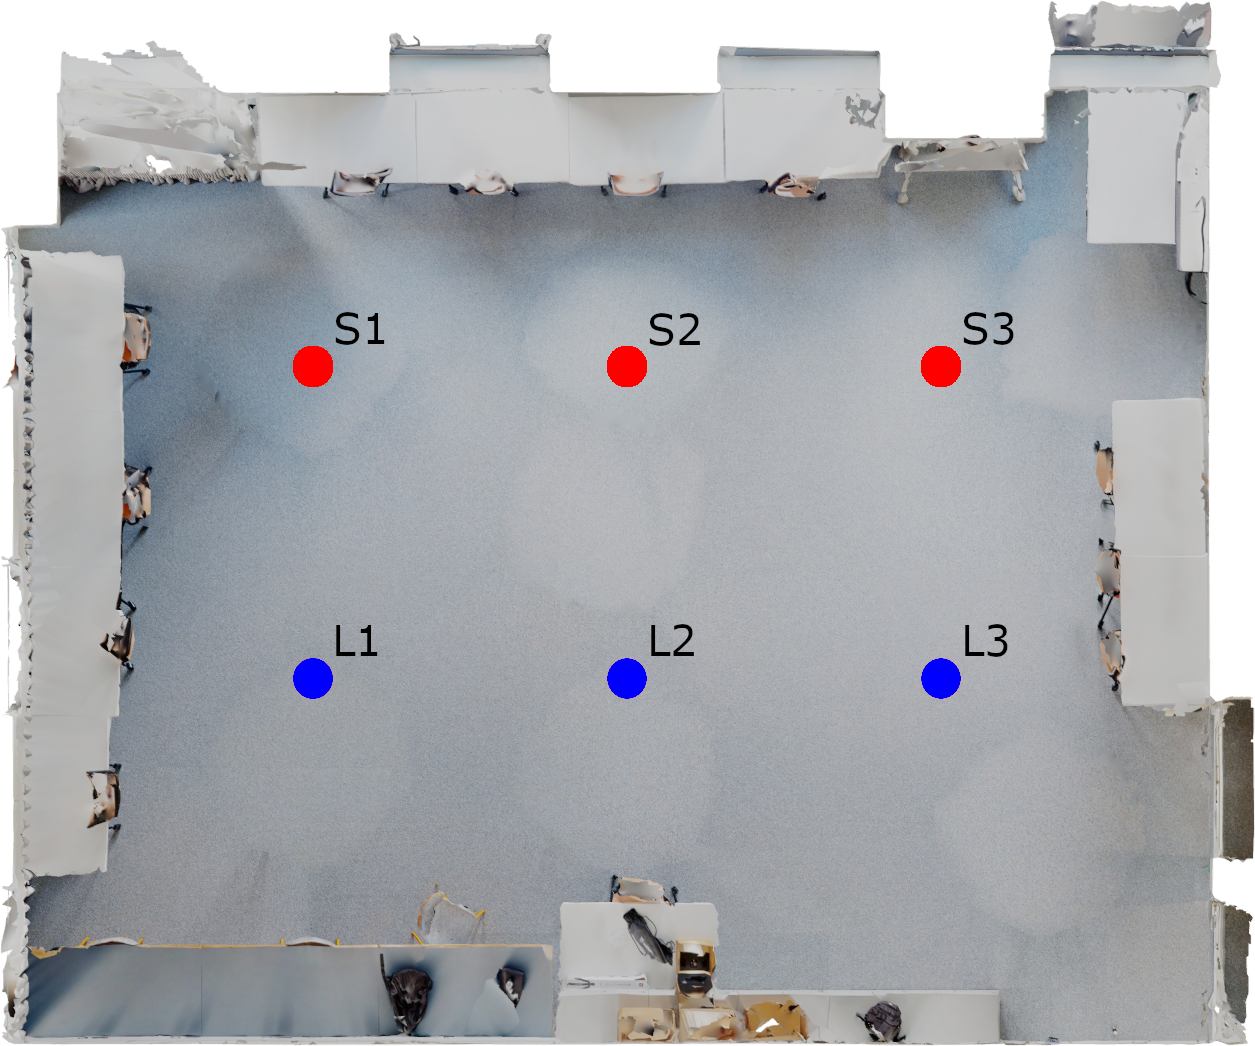
\includegraphics[width=\textwidth]{grid-a}
       \caption{Grid A}
       \label{fig:grid-a-probes}
    \end{subfigure}
    \begin{subfigure}[t]{0.45\textwidth}
       \centering
       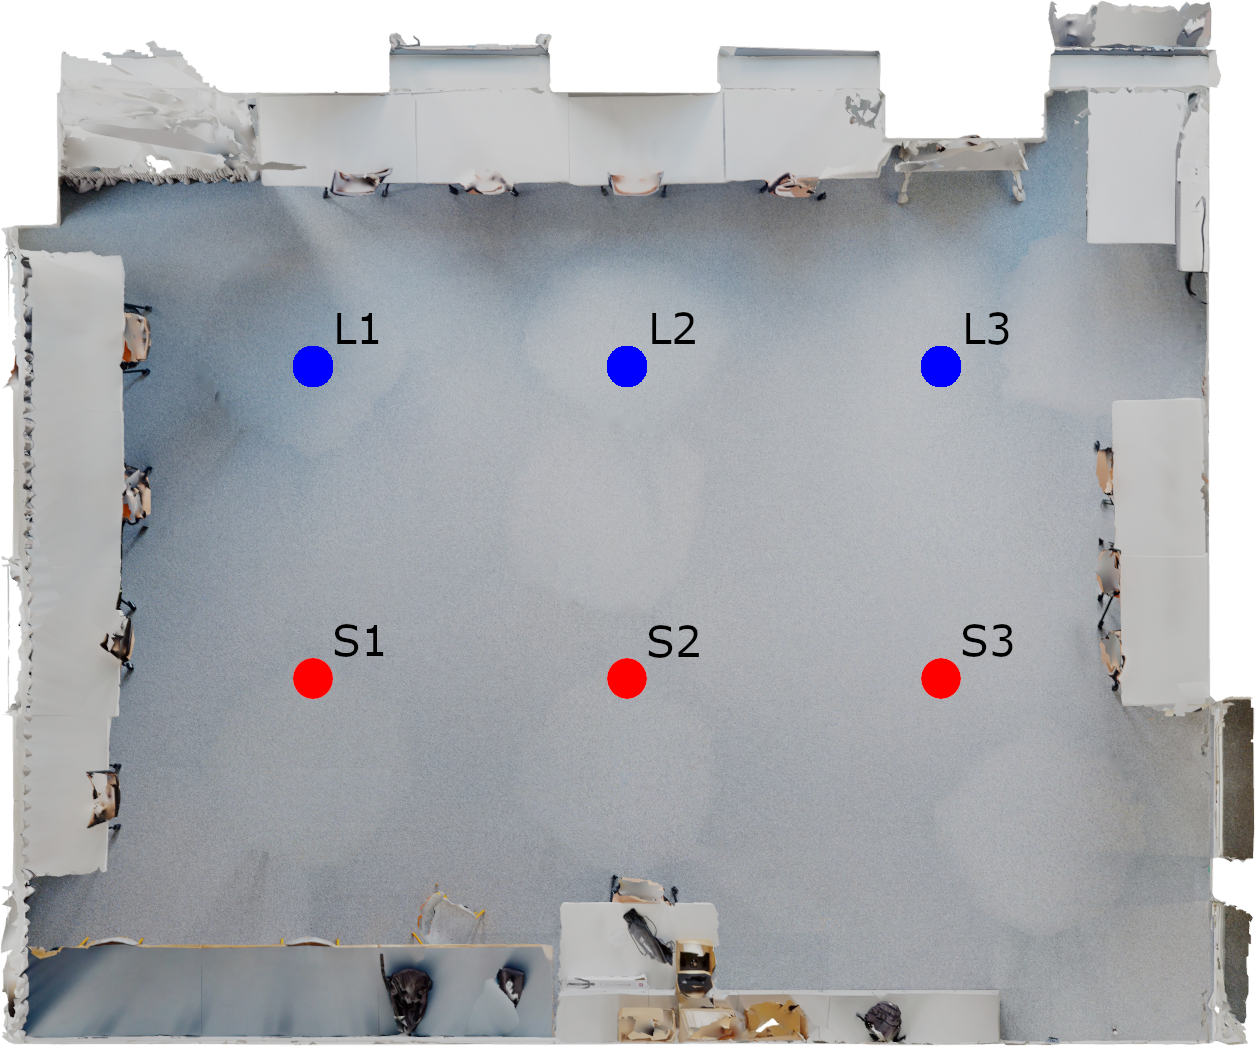
\includegraphics[width=\textwidth]{grid-b}
       \caption{Grid B}
       \label{fig:grid-b-probes}
    \end{subfigure}
\caption{Source-Listener location points in the recording environment. RIR are recorded between source positions \textbf{S1, S2, S3} and listener positions \textbf{L1, L2, L3}; these pairs are then inverted, obtaining uniformly spaces probe points across the soundfield.}
\label{fig:rir-recording-probes}
\end{figure}

\subsection{Apparatus and Test Procedure}
\label{sec:acoustic_eval_procedure}
The experimental evaluation apparatus includes measurement equipment for capturing the acoustic space, space-capturing techniques to generate a virtual reconstruction of the lecture room, and the geometrical acoustics-based rendering pipeline illustrated.


\subsubsection{Real Soundfield Measurements}
\label{sec:real_soundfield_measurement}
Following standard acoustic measurement procedures described by the British Standard \cite{bs3382-1}, sampling a space uniformly by recording measurement signals emitted by a speaker and recorded by a microphone. The test uses a dodecahedron speaker to fit the emitter directionality requirements established by the BS 3382-1 and to maximise the excitation of the soundfield, a Nor276 Dodecahedron Loudspeaker\footnote{\url{https://web2.norsonic.com/product_single/dodecahedron-loudspeaker-nor276/}} driven by a Nor282 Amplifier\footnote{\url{https://web2.norsonic.com/product_single/power-amplifier-nor282/}}. A Focusrite Scarlett 18i8\footnote{\url{https://focusrite.com/products/scarlett-18i8}} microphone pre-amplifier and Analogue/Digital, Digital/Analogue Converter is used to emit a $30s$ long logarithmically swept sine signal $x$ ranging from $20Hz$ to $20kHz$. A Rode NT-SF1\footnote{\url{https://rode.com/en/microphones/360-ambisonic/nt-sf1}} flat-frequency response ($\pm4dB$ between $20Hz$ to $20kHz$) ambisonic microphone captures the swept sine emitted by the speaker via the Focusrite Scarlett 18i8. \par
The same procedure was repeated for all source-listener position pairs illustrated in Figure~\ref{fig:rir-recording-probes} across both grid formations: the speaker on the red dot and the microphone is placed on the blue dot, facing the speaker; the swept sine signal is recorded $y$, recovering the response $h$ by convolving it to the time reversal sequence of the original sweep, $h(t) = y(t) * x(-t)$, as demonstrated by \cite{farina07}. \par

\subsubsection{Simulated Soundfield Measurements}
The lecture room was captured using a Matterport Pro3\footnote{\url{https://matterport.com/pro3}} space-scanning camera, generating a triangulated 3D mesh that the geometry handling system of proposed acoustic rendering pipeline uses to construct a scene BVH for geometrical operations of the ray tracer.\par
The acoustic rendering pipeline is deployed on the scene, defining two $0.5m$ radius spheres as source and receiver volumes and emitting $3*10^5$ rays, allowing $4$ orders of reflections. RIRs are constructed in about $60s$ with an unoptimised and unparallelised implementation running on the Unity game engine scripting runtime. The same procedure described in the previous Section is repeated. \par

\subsection{Results}
RIRs obtained from both real and simulated soundfields are reported in Figures~\ref{fig:rir-comparisons-grid-a}, \ref{fig:rir-comparisons-grid-a2}, \ref{fig:rir-comparisons-grid-b}, \ref{fig:rir-comparisons-grid-b2}; these plots show Simulated and Measured RIRs in the first and columns, respectively, reporting comparisons of decay curves obtained from smoothed analytic signals from the absolute value of a Hilbert transform of the respective RIR. The Measured RIRs have around $45dB$ of signal-to-noise ratio, and the Simulated ones are over $120dB$. \par
From these responses, metrics, shown in Table \ref{tab:rt-metrics}, describing the acoustic space are computed, including the T\textsubscript{30} reverberation, C\textsubscript{50} clarity and D\textsubscript{50} definition indexes that relate to factors of sound transmissions occurring within the space, affecting tasks such as speech intelligibility or perception of spatial features of sound sources via auditory information. Changes in clarity and definition parameters are observed as a function of distance from the source across all listeners; see Table~\ref{tab:source-listener-distances} for distance values. \par
The T\textsubscript{30} reverberation metric is obtained from the computed analytic signal, and the D\textsubscript{50} and C\textsubscript{50} are computed from the responses, following the BS \cite{bs3382-1} definitions,
\begin{equation}
    D_{50} = \frac{\bigint_{0}^{0.05} p^2(t)\textrm{d}t}{\bigint_{0}^{\infty} p^2(t)\textrm{d}t}\quad \textrm{and} \quad C_{50} = 10log_{10} \left( \frac{D_{50}}{1-D_{50}} \right)\textrm{,}
\end{equation}
where $p$ is the magnitude of sound events expressed by the response. Additionally, the sound strength metric $G$ between a $near$ and $far$ sound source is defined as:
\begin{equation}
    G = 10 log_{10} \frac{\bigint_{0}^{\infty} p_{near}^2(t)\textrm{d}t}{\bigint_{0}^{\infty} p_{far}^2(t)\textrm{d}t} \textrm{;}
\end{equation}
$G$ scores are reported in Table~\ref{tab:g-scores}.

% \begin{table}[h]
% \resizebox{\textwidth}{!}{%
% \begin{tabular}{@{}lllllll@{}}
% \toprule
% Position Pair & T\textsubscript{30} Simulated & T\textsubscript{30} Real & C\textsubscript{50} Simulated & C\textsubscript{50} Real & D\textsubscript{50} Simulated & D\textsubscript{50} Real \\ \midrule
% S1 L1         & 0.12                          & 0.43                     & 4.33                          & 3.2                      & 0.27                          & 0.32                     \\
% S1 L2         & 0.12                          & 0.41                     & 2.96                          & 3.33                     & 0.34                          & 0.32                     \\
% S1 L3         & 0.12                          & 0.41                     & 2.74                          & 2.45                     & 0.35                          & 0.36                     \\
% S2 L1         & 0.12                          & 0.45                     & 5.81                          & 3.4                      & 0.21                          & 0.31                     \\
% S2 L2         & 0.12                          & 0.43                     & 2.02                          & 3.16                     & 0.39                          & 0.33                     \\
% S2 L3         & 0.12                          & 0.43                     & 3.9                           & 1.74                     & 0.29                          & 0.4                      \\
% S3 L1         & 0.11                          & 0.42                     & 1.46                          & 2.45                     & 0.42                          & 0.36                     \\
% S3 L2         & 0.11                          & 0.47                     & 1.72                          & 2.96                     & 0.4                           & 0.34                     \\
% S3 L3         & 0.12                          & 0.45                     & 1.92                          & 2.71                     & 0.39                          & 0.35                     \\ \bottomrule
% \end{tabular}%
% }
% \caption{Standard acoustic metrics collected across source-receiver position pairs for Grid A, see Figure~\ref{fig:grid-a-probes}. The T\textsubscript{30} reverberation time, C\textsubscript{50} clarity index, and D\textsubscript{50} definition index are dependent on the magnitude and distribution of acoustic energy expressed by the respective RIR. In this case, simulated and measured RIRs are compared.}
% \label{tab:grid-a-metrics}
% \end{table}

% \begin{table}[]
% \begin{tabular}{@{}lllllll@{}}
% \toprule
% Position Pair & T\textsubscript{30} Simulated & T\textsubscript{30} Real & C\textsubscript{50} Simulated & C\textsubscript{50} Real & D\textsubscript{50} Simulated & D\textsubscript{50} Real \\ \midrule
% S1 L1         & 0.12                        & 0.44                   & 3.74                        & 2.43                   & 0.30                        & 0.37                   \\
% S1 L2         & 0.10                        & 0.40                   & 2.13                        & 2.83                   & 0.38                        & 0.34                   \\
% S1 L3         & 0.11                        & 0.41                   & 2.80                        & 2.45                   & 0.34                        & 0.36                   \\
% S2 L1         & 0.11                        & 0.43                   & 9.02                        & 2.95                   & 0.11                        & 0.34                   \\
% S2 L2         & 0.11                        & 0.49                   & 7.96                        & 3.93                   & 0.14                        & 0.29                   \\
% S2 L3         & 0.10                        & 0.49                   & 3.33                        & 3.62                   & 0.32                        & 0.30                   \\
% S3 L1         & 0.11                        & 0.45                   & 6.24                        & 3.57                   & 0.19                        & 0.31                   \\
% S3 L2         & 0.10                        & 0.46                   & 2.71                        & 2.42                   & 0.35                        & 0.36                   \\
% S3 L3         & 0.10                        & 0.39                   & 2.76                        & 2.88                   & 0.35                        & 0.34                   \\ \bottomrule
% \end{tabular}
% \caption{Acoustic metrics relating to Grid B positions as illustrated in Table~\ref{tab:grid-a-metrics}.}
% \label{tab:grid-b-metrics}
% \end{table}

% Please add the following required packages to your document preamble:
% \usepackage{booktabs}
% \usepackage{multirow}
\begin{table}[]
\centering
\begin{tabular}{@{}lllllllllll@{}}
\toprule
  Grid & 
  Pos. Pair &
  T\textsubscript{30} Sim. &
  T\textsubscript{30} Real &
  C\textsubscript{50} Sim.  &
  C\textsubscript{50} Real &
  D\textsubscript{50} Sim. &
  D\textsubscript{50} Real \\ \midrule
\multirow{9}{*}{A} & \textbf{S1 L1}      & 0.12 & 0.43 & 4.33 & 3.20 & 0.27 & 0.32 \\
                        & \textbf{S1 L2} & 0.12 & 0.41 & 2.96 & 3.33 & 0.34 & 0.32 \\
                        & \textbf{S1 L3} & 0.12 & 0.41 & 2.74 & 2.45 & 0.35 & 0.36 \\
                        & \textbf{S2 L1} & 0.12 & 0.45 & 5.81 & 3.40 & 0.21 & 0.31 \\
                        & \textbf{S2 L2} & 0.12 & 0.43 & 2.02 & 3.16 & 0.39 & 0.33 \\
                        & \textbf{S2 L3} & 0.12 & 0.43 & 3.90 & 1.74 & 0.29 & 0.40 \\
                        & \textbf{S3 L1} & 0.11 & 0.42 & 1.46 & 2.45 & 0.42 & 0.36 \\
                        & \textbf{S3 L2} & 0.11 & 0.47 & 1.72 & 2.96 & 0.40 & 0.34 \\
                        & \textbf{S3 L3} & 0.12 & 0.45 & 1.92 & 2.71 & 0.39 & 0.35 \\ \cmidrule(l){1-8}
\multirow{9}{*}{B} & \textbf{S1 L1}      & 0.12 & 0.44 & 3.74 & 2.43 & 0.30 & 0.37 \\
                        & \textbf{S1 L2} & 0.10 & 0.40 & 2.13 & 2.83 & 0.38 & 0.34 \\
                        & \textbf{S1 L3} & 0.11 & 0.41 & 2.80 & 2.45 & 0.34 & 0.36 \\
                        & \textbf{S2 L1} & 0.11 & 0.43 & 9.02 & 2.95 & 0.11 & 0.34 \\
                        & \textbf{S2 L2} & 0.11 & 0.49 & 7.96 & 3.93 & 0.14 & 0.29 \\
                        & \textbf{S2 L3} & 0.10 & 0.49 & 3.33 & 3.62 & 0.32 & 0.30 \\
                        & \textbf{S3 L1} & 0.11 & 0.45 & 6.24 & 3.57 & 0.19 & 0.31 \\
                        & \textbf{S3 L2} & 0.10 & 0.46 & 2.71 & 2.42 & 0.35 & 0.36 \\
                        & \textbf{S3 L3} & 0.10 & 0.39 & 2.76 & 2.88 & 0.35 & 0.34 \\ \cmidrule(l){1-8} 
\end{tabular}
\caption{Standard acoustic metrics collected across source-receiver position pairs for Grid A and B, see Figure~\ref{fig:rir-recording-probes}. The T\textsubscript{30} reverberation time, C\textsubscript{50} clarity index, and D\textsubscript{50} definition index are dependent on the magnitude and distribution of acoustic energy expressed by the respective RIR. In this case, simulated and measured RIRs are compared.}
\label{tab:rt-metrics}
\end{table}

\begin{table}[]
\begin{tabular}{@{}llllllll@{}}
\toprule
Grid & Pair & T\textsubscript{30} Err. & $T_{30}$ & C\textsubscript{50} Err. & $C_{50}$ & D\textsubscript{50} Err. &  $D_{50}$ \\ \midrule
    \multirow{9}{*}{A}  & \textbf{S1 L1} & 0.31  & \multirow{3}{*}{$\mu = 0.32$} & -1.13 & \multirow{3}{*}{$\mu = -0.16$} & 0.05  & \multirow{3}{*}{$\mu = 0.00$} \\
       & \textbf{S1 L2} & 0.29 &                       & 0.37  &                        & -0.02 &                       \\
       & \textbf{S1 L3} & 0.29 &                       & -0.29 &                        & 0.01  &                       \\
       & \textbf{S2 L1} & 0.33 & \multirow{3}{*}{$\sigma = 0.02$} & -2.41 & \multirow{3}{*}{$\sigma = 1.34$}  & 0.10  & \multirow{3}{*}{$\sigma = 0.06$} \\
       & \textbf{S2 L2} & 0.31 &                       & 1.14  &                        & -0.06 &                       \\
       & \textbf{S2 L3} & 0.31 &                       & -2.16 &                        & 0.11  &                       \\
       & \textbf{S3 L1} & 0.31 & \multirow{3}{*}{$\scriptstyle{MSE}~=~\normalsize{0.10}$} & 0.99  & \multirow{3}{*}{$\scriptstyle{MSE}~=~1.82$}  & -0.06 & \multirow{3}{*}{$\scriptstyle{MSE}~=~0.00$} \\
       & \textbf{S3 L2} & 0.36 &                       & 1.24  &                        & -0.06 &                       \\
       & \textbf{S3 L3} & 0.33 &                       & 0.79  &                        & -0.04 &                       \\ \cmidrule(l){1-8}
    \multirow{9}{*}{B}& \textbf{S1 L1} & 0.32 & \multirow{3}{*}{$\mu = 0.33$} & -1.31 & \multirow{3}{*}{$\mu = -1.51$} & 0.07  & \multirow{3}{*}{$\mu = 0.06$} \\ 
       & \textbf{S1 L2} & 0.30 &                       & 0.70  &                        & -0.04 &                       \\
       & \textbf{S1 L3} & 0.30 &                       & -0.35 &                        & 0.02  &                       \\
       & \textbf{S2 L1} & 0.32 & \multirow{3}{*}{$\sigma = 0.04$} & -6.07 & \multirow{3}{*}{$\sigma = 2.29$}  & 0.23  & \multirow{3}{*}{$\sigma = 0.09$} \\
       & \textbf{S2 L2} & 0.38 &                       & -4.03 &                        & 0.15  &                       \\
       & \textbf{S2 L3} & 0.39 &                       & 0.29  &                        & -0.02 &                       \\
       & \textbf{S3 L1} & 0.34 & \multirow{3}{*}{$\scriptstyle{MSE}~=~0.11$} & -2.67 & \multirow{3}{*}{$\scriptstyle{MSE}~=~6.97$}  & 0.12  & \multirow{3}{*}{$\scriptstyle{MSE}~=~0.01$} \\
       & \textbf{S3 L2} & 0.36 &                       & -0.29 &                        & 0.01  &                       \\
       & \textbf{S3 L3} & 0.29 &                       & 0.12  &                        & -0.01 &                       \\ \cmidrule(r){1-8}
\end{tabular}

\caption{Descriptive statistics.}
\label{tab:rt-metrics-stats}
\end{table}

% Please add the following required packages to your document preamble:
% \usepackage{booktabs}
% \usepackage{graphicx}
\begin{table}[]
\centering
\begin{tabular}{@{}lllll@{}}
\toprule
Receiver Position & \multicolumn{2}{l}{Grid A} & \multicolumn{2}{l}{Grid B} \\ \midrule
                  & Simulated     & Real       & Simulated      & Real      \\
L1                & -1.156        & 0.505      & 1.607          & -2.89     \\
L3                & -2.169        & -2.203     & 2.022          & -3.39     \\ \bottomrule
\end{tabular}%
\caption{G Sound strength values (dB) across the two source-listener position pair grids, see Figure~\ref{fig:rir-recording-probes}. For each grid, two receiver positions are used to measure the sound strength by computing the ratio of instantaneous energy between a near and a far source. Hence, for \textbf{L1} the ratio of energy between \textbf{S1} and \textbf{S3} is measured (near and far, respectively), and for \textbf{L3}, is measured between \textbf{S3} and  \textbf{S1}.}
\label{tab:g-scores}
\end{table}

\begin{figure}
    \centering
    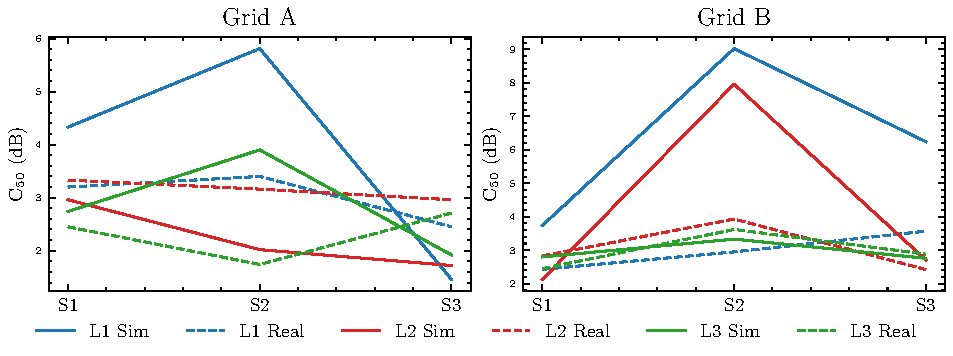
\includegraphics[width=1\linewidth]{c50}
    \caption{C\textsubscript{50} index values for both the simulated and measured soundfield, observed over distance from the sound source.}
    \label{fig:c50comparison}
\end{figure}
\begin{figure}
    \centering
    \includegraphics[width=1\linewidth]{d50}
    \caption{D\textsubscript{50} index values for both the simulated and measured soundfield over distance from the sound source.}
    \label{fig:d50comparison}
\end{figure}

% Grid A
\begin{figure}
    \centering
    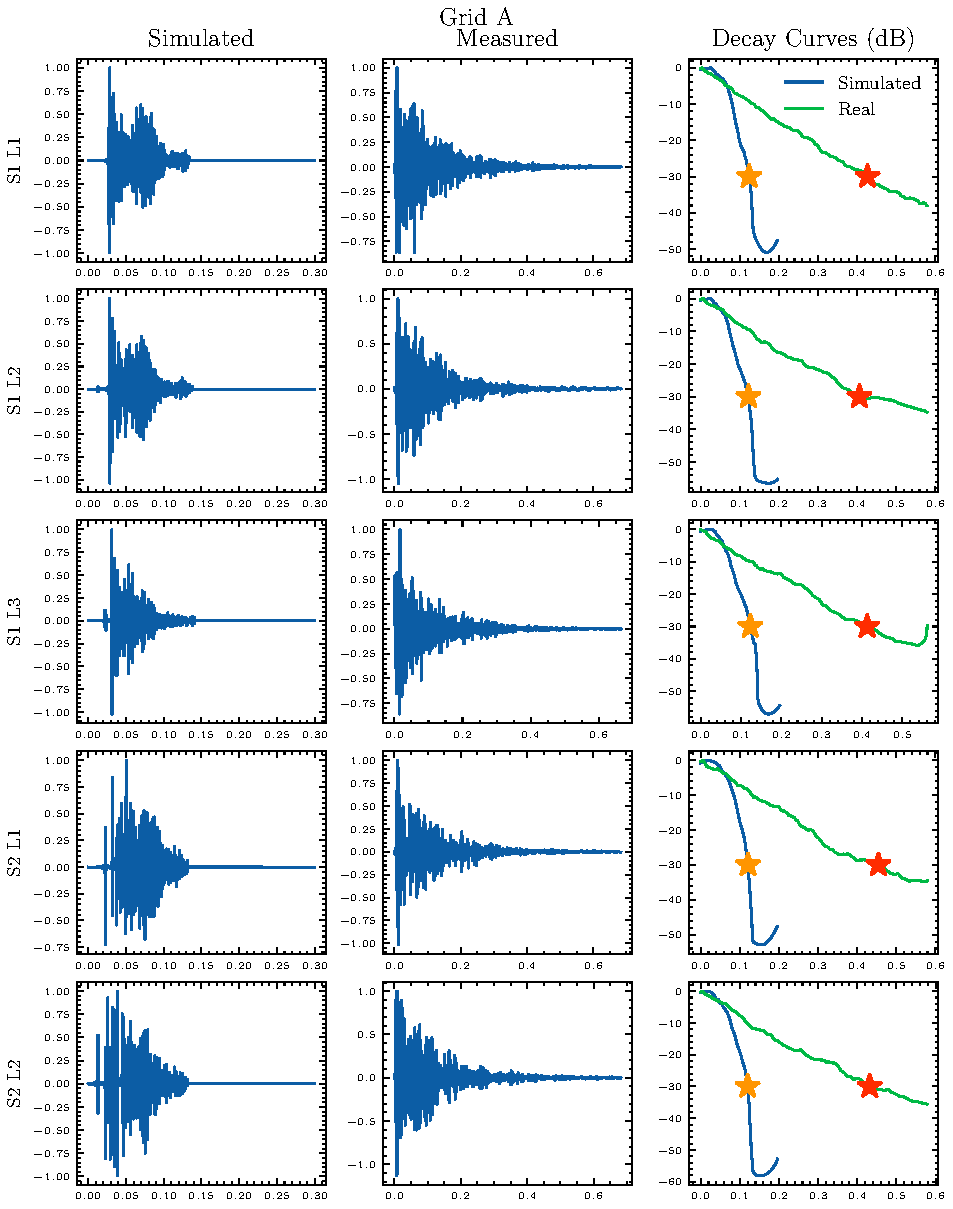
\includegraphics[width=1\linewidth]{real_synthetic_rir}
    \caption{Time-domain representation of responses, as magnitude over time (s), obtained from simulations of the soundfield of a virtual reconstruction of a lecture room, first column, across permutations of source-listener position pairs illustrated in Figure~\ref{fig:grid-a-probes}, rows. These are compared to responses obtained from acoustic measurements of the physical space, second column. The third column shows comparisons of the acoustic energy, as attenuation (dB) over time (s), decay across the two responses with overlaid light, yellow star and dark, red star indicating T\textsubscript{30} values for simulated and measured responses, respectively.}
    \label{fig:rir-comparisons-grid-a}
\end{figure}
% Grid A pt 2
\begin{figure}
    \centering
    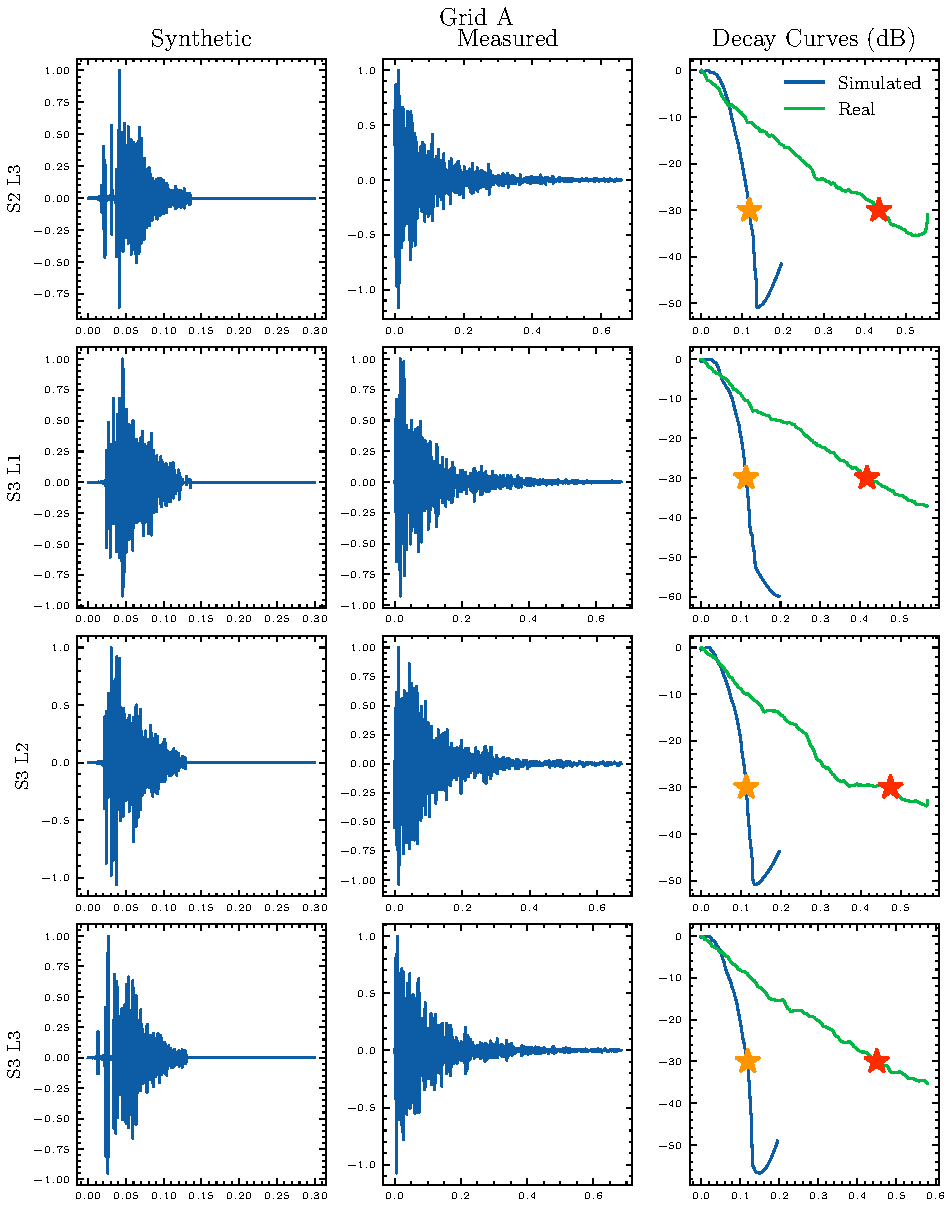
\includegraphics[width=1\linewidth]{real_synthetic_rir_cont}
    \caption{Continuation of rows from Figure~\ref{fig:rir-comparisons-grid-a}, showing remaining source-listener position pairs.}
    \label{fig:rir-comparisons-grid-a2}
\end{figure}
% Grid B
\begin{figure}
    \centering
    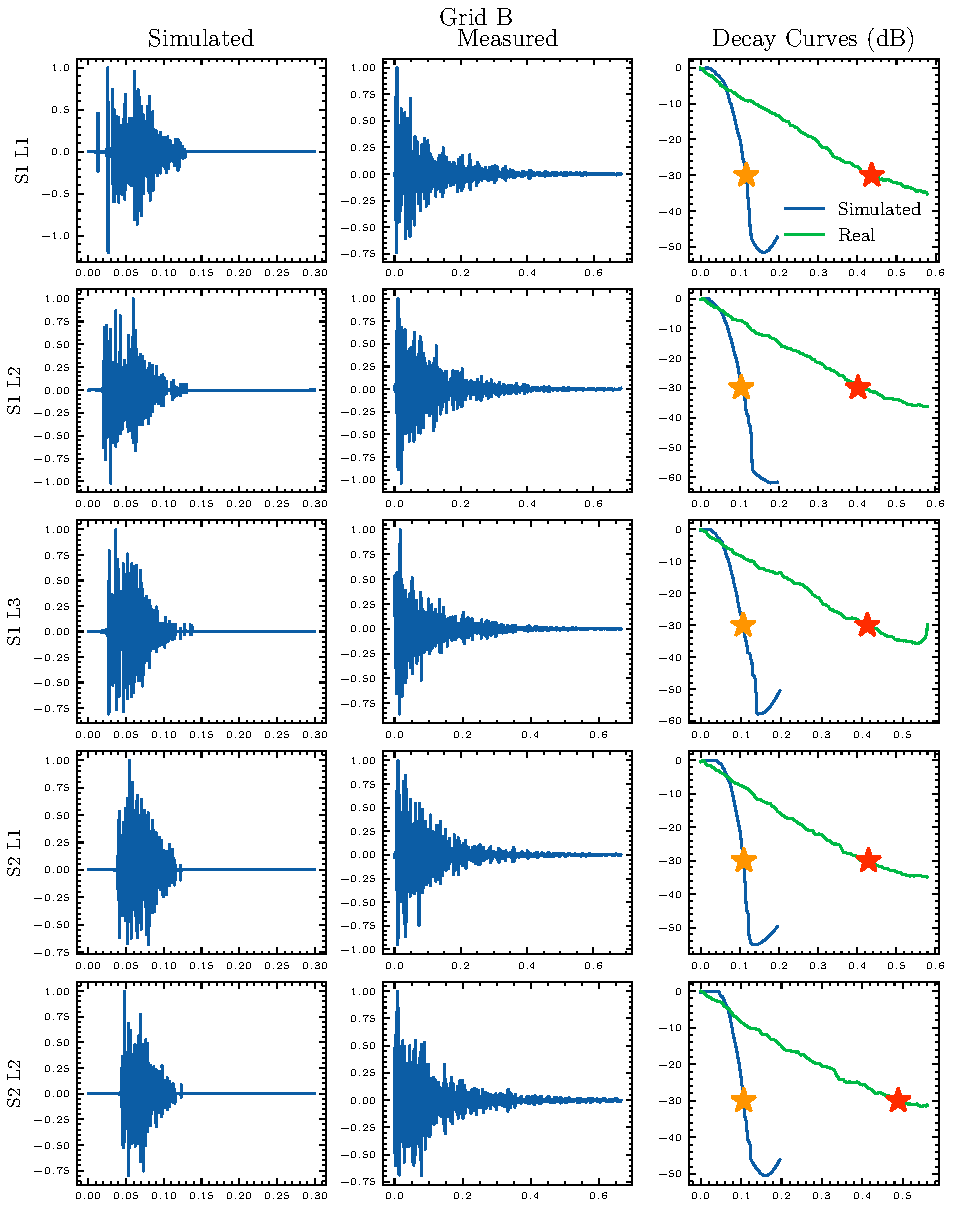
\includegraphics[width=1\linewidth]{real_synthetic_rir_b}
    \caption{Continuation of rows from Figure~\ref{fig:rir-comparisons-grid-a}, showing responses from position pairs illustrated in Figure~\ref{fig:grid-b-probes}.}
    \label{fig:rir-comparisons-grid-b}
\end{figure}
% Grid B pt 2
\begin{figure}
    \centering
    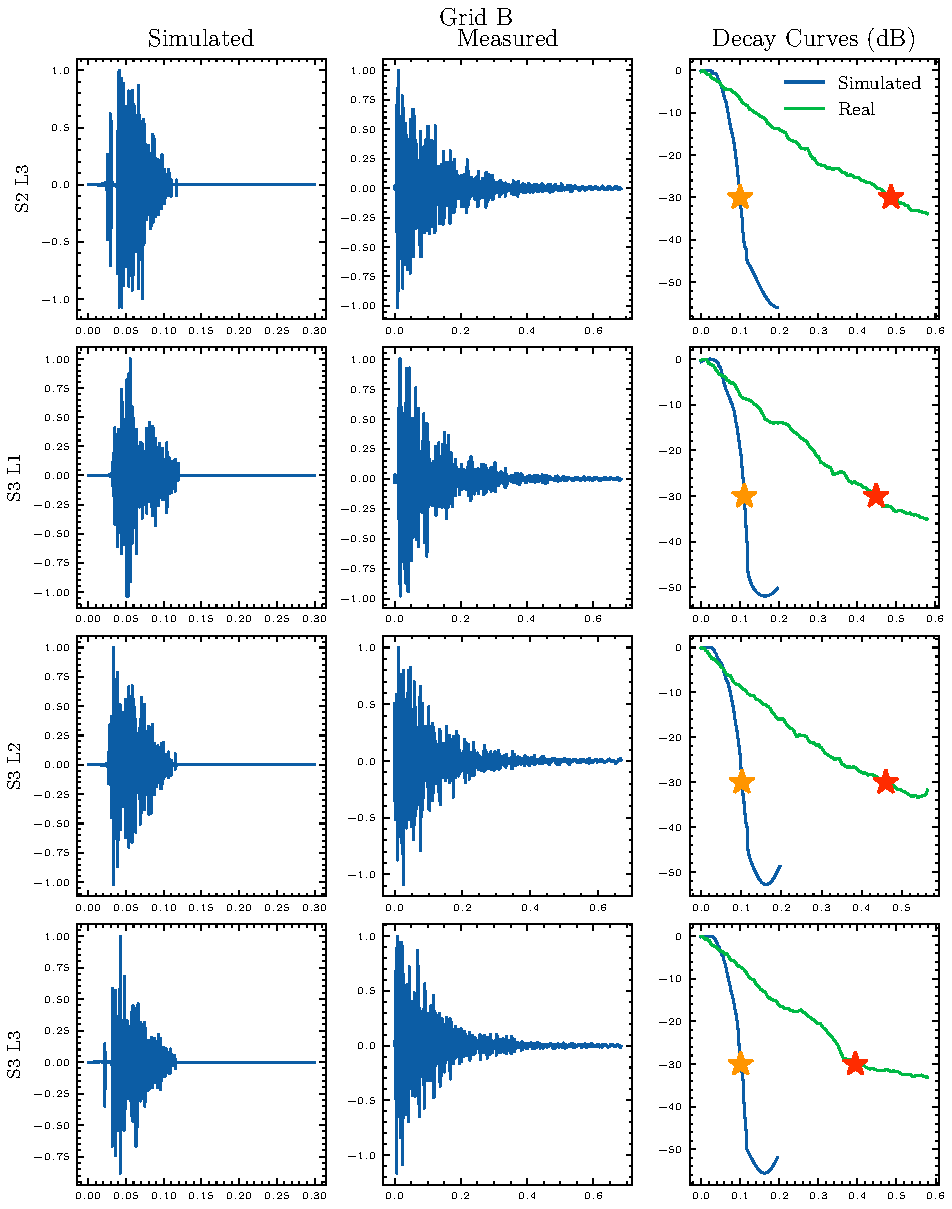
\includegraphics[width=1\linewidth]{real_synthetic_rir_bcont}
    \caption{Continuation of rows from Figure~\ref{fig:rir-comparisons-grid-b}, showing remaining source-listener position pairs.}
    \label{fig:rir-comparisons-grid-b2}
\end{figure}



\subsection{Discussion}
Reverberation is the parameter relating to the acoustic soundfield where the largest discrepancy between the simulated and real responses is observed, as shown in Tables~\ref{tab:rt-metrics} and \ref{tab:rt-metrics-stats}. By observing decay lines fit over the responses shown in Figures~\ref{fig:rir-comparisons-grid-a} to \ref{fig:rir-comparisons-grid-b2}, the acoustic rendering pipeline has a sharper energy decay, with limited capabilities in reproducing late energy transfers from emitter to receiver. The limited resolution of low-frequency energy in the simulated soundscape contributes to the reverberation discrepancy from the ground truth caused by incorrect modelling of directionality profiles of radiating waves. Geometrical acoustics pipelines can be integrated with modern acoustic radiance modelling techniques, as demonstrated by \cite{siltanen2010room}. Despite the measured reverberation time error in the simulated soundfield, the improved pipeline demonstrates an extensive improvement from the first prototype, as shown in Table~\ref{tab:ism_scene_scores}. In addition, the limitation of the ISM model in adapting to architectural features of the scene geometry. \par
Comparing the measured $T_{30}$ error, using reverberation as a determinant of perceptual aspects of sound transmissions in a soundfield, the proposed geometrical acoustics-based rendering pipeline aligns with state-of-the-art and modern realistic methods for acoustic rendering. As discussed in Section~\ref{sec:lr-visual-acoustic-mapping}, modern rendering pipelines adopt learned Generative Adversarial Neural Networks to determine reverberation features of multi-modal representations of complex scenes. The proposed acoustic rendering pipeline estimates reverberation with similar or better accuracy compared to \cite{Singh_2021_ICCV}'s work. Such error is acceptable even when considering advanced realistic multi-modal pipelines such as \cite{schissler2014high}'s work. \par


\section{Conclusions}
The ISM prototype was used to test the integration of material recognition systems into acoustic rendering pipelines. 
The ray tracer implementation provides important insights into the implementation of an acoustic rendering pipeline that can be streamlined for interactive applications. Whilst there are inherent limitations of the acoustic modelling technique, the improved design can still approximate basic acoustic phenomena such as reverberation or reflections.